\documentclass[a4paper,11pt,oneside]{book}

% packages 
\usepackage{arsclassica}    % fancy layout
\usepackage[english]{babel}\addto{\captionsenglish}{\renewcommand{\bibname}{References}}
\usepackage{caption}         % figure captions
\usepackage[square,numbers,super,sort&compress]{natbib}  % bibliography style
\usepackage[cc]{titlepic}    % enable logo on title page
\usepackage{graphicx}       % logo related

% Margins for pretty version ::
%\usepackage[pass]{geometry}
% Margins for university regulations ::
\usepackage[top=2cm, bottom=4cm, left=4cm, right=2.5cm]{geometry}
\usepackage{setspace}
\onehalfspacing

\usepackage{standalone}
\standalonetrue

% don't hang captions
\captionsetup{format=plain}

% bibliography
\bibliographystyle{../thesis}

\graphicspath {{../figs/}}

\begin{document}

%\maketitle

\chapter{Chromatin domain boundaries}\label{chap:boundaries}

\section{Introduction}

A succession of studies have defined chromatin domains of different types, for example: A and B chromosome compartments;\cite{Lieberman2009} topologically associating domains (TADs);\cite{Dixon2012} contact and loop domains;\cite{Rao2014} physical domains;\cite{Sexton2012, Hou2012} and others.\cite{Filippova2014} The existence of these domains necessitates "boundary regions" either between consecutive domains or bookending more separated domains, however the functional relevance of said boundary regions is still open to debate.

In their study of topological domains, \citet{Dixon2012} identified average enrichments over TAD boundary regions in both human and mouse for various features including CTCF and PolII. Boundaries were also enriched for signs of active transcription, such as with the histone modification H3k36me3.\cite{Dixon2012} These results, coupled with an observable enrichment for promoters at domain boundaries, have lead to the theory that boundaries may act as an additional layer of transcriptional control.\cite{Sexton2015} However an alternative theory  is that if chromatin domains represent co-regulatory regions as is widely thought,\cite{LeDily2014, Nora2013, Sexton2015} boundaries themselves could be mere side-effects and as such of limited biological interest.

An obvious experiment to resolve these opposing theories would be to delete a predicted boundary region and test for local changes in both contacts and expression. Such an experiment was performed on a region of the human X-chromosome containing the genes encoding the dosage-compensation long non-coding RNAs \emph{Xist} and \emph{Tsix}, which are separated by a TAD boundary.\cite{Nora2012} This study found that while histone modifications within the body of a TAD could be removed without affecting overall domain structure, deletion of a boundary did have an effect and led to increased intradomain contacts.\cite{Nora2012} Surprisingly however, the two domains did not completely merge, lending credence to the alternative theory that TADs may be centrally constrained, rather than by their borders.\cite{Nora2012} 

A recent experiment used CRISPR genome editing to link TAD boundary changes with limb development disorders,\cite{Lupianez2015} indicating that boundary changes could provide an underlying explanation for pathogenic non-coding structural variants.\cite{Ren2015} Similarly, domain boundaries on \emph{C. elegans} X-chromosomes were found to be weakened following the disruption of condensin binding sites.\cite{Crane2015} Together these studies suggest a complex scenario whereby TAD boundaries are an important structural feature, yet do not fully explain domain partitioning.

%Computational analysis of boundaries has emerged during the time this work was completed. Border "strength", here defined by the ratio of total intra:inter-domain contacts, was found to correlate with increased occupancy of a combination of bound architectural proteins.\cite{VanBortle2014}

Many questions remain about chromatin boundaries. For example, are the enrichments reported in \citet{Dixon2012} persistent across cell types and how do they compare across organisation strata, such as compartments and TADs? Through computational analysis of the set of boundaries re-called from published datasets, we can investigate these questions and probe boundary enrichments across a broad array of locus-level chromatin features.

\section{Boundary analysis}\label{sec:boundaryenrichments}

The mammalian genome is organized into topologically associating domains (TADs), predominantly self-interacting chromatin domains, with boundary regions reportedly associated with pronounced peaks and troughs of particular features within 500 kb of the predicted boundary.\cite{Dixon2012} Exploration of this phenomenon using a set of 24 mouse ESC chromatin features (and a smaller number of human ESC features) revealed enrichment peaks of CTCF, H3K4me3 and H3K36me3, as well as a pronounced dip in H3K9me3, suggesting that high levels of transcription may contribute to boundary formation.\cite{Dixon2012} However, the peaks and dips of these features lacked any estimates of statistical significance. It was also unclear whether other features might show unusual patterns in TAD boundary regions, and how the constellation of features involved might vary between cell types. Moreover, the features associated with boundaries separating A and B compartments calculated from Hi-C eigenvectors have not been studied to our knowledge. The datasets assembled here, consisting of 35 matched chromatin features across three cell types, allow us to conduct the first comparative study of the constituents of human TAD and compartment boundary regions.

\subsection{TAD boundaries}

We derived TAD boundaries from uniformly reprocessed Hi-C data (Chapter \ref{chap:hiccomparison}) according to established methods (see Methods \ref{meth:tadcalling}) for all three cell types under study. We then sought evidence for significantly enriched or depleted features at TAD boundary regions using a conservative approach (a nonparametric statistical test and Bonferroni multiple testing correction, see Methods \ref{meth:tadbounds}).

\begin{figure}
\begin{center} 
\makebox[\textwidth][c]{ 
	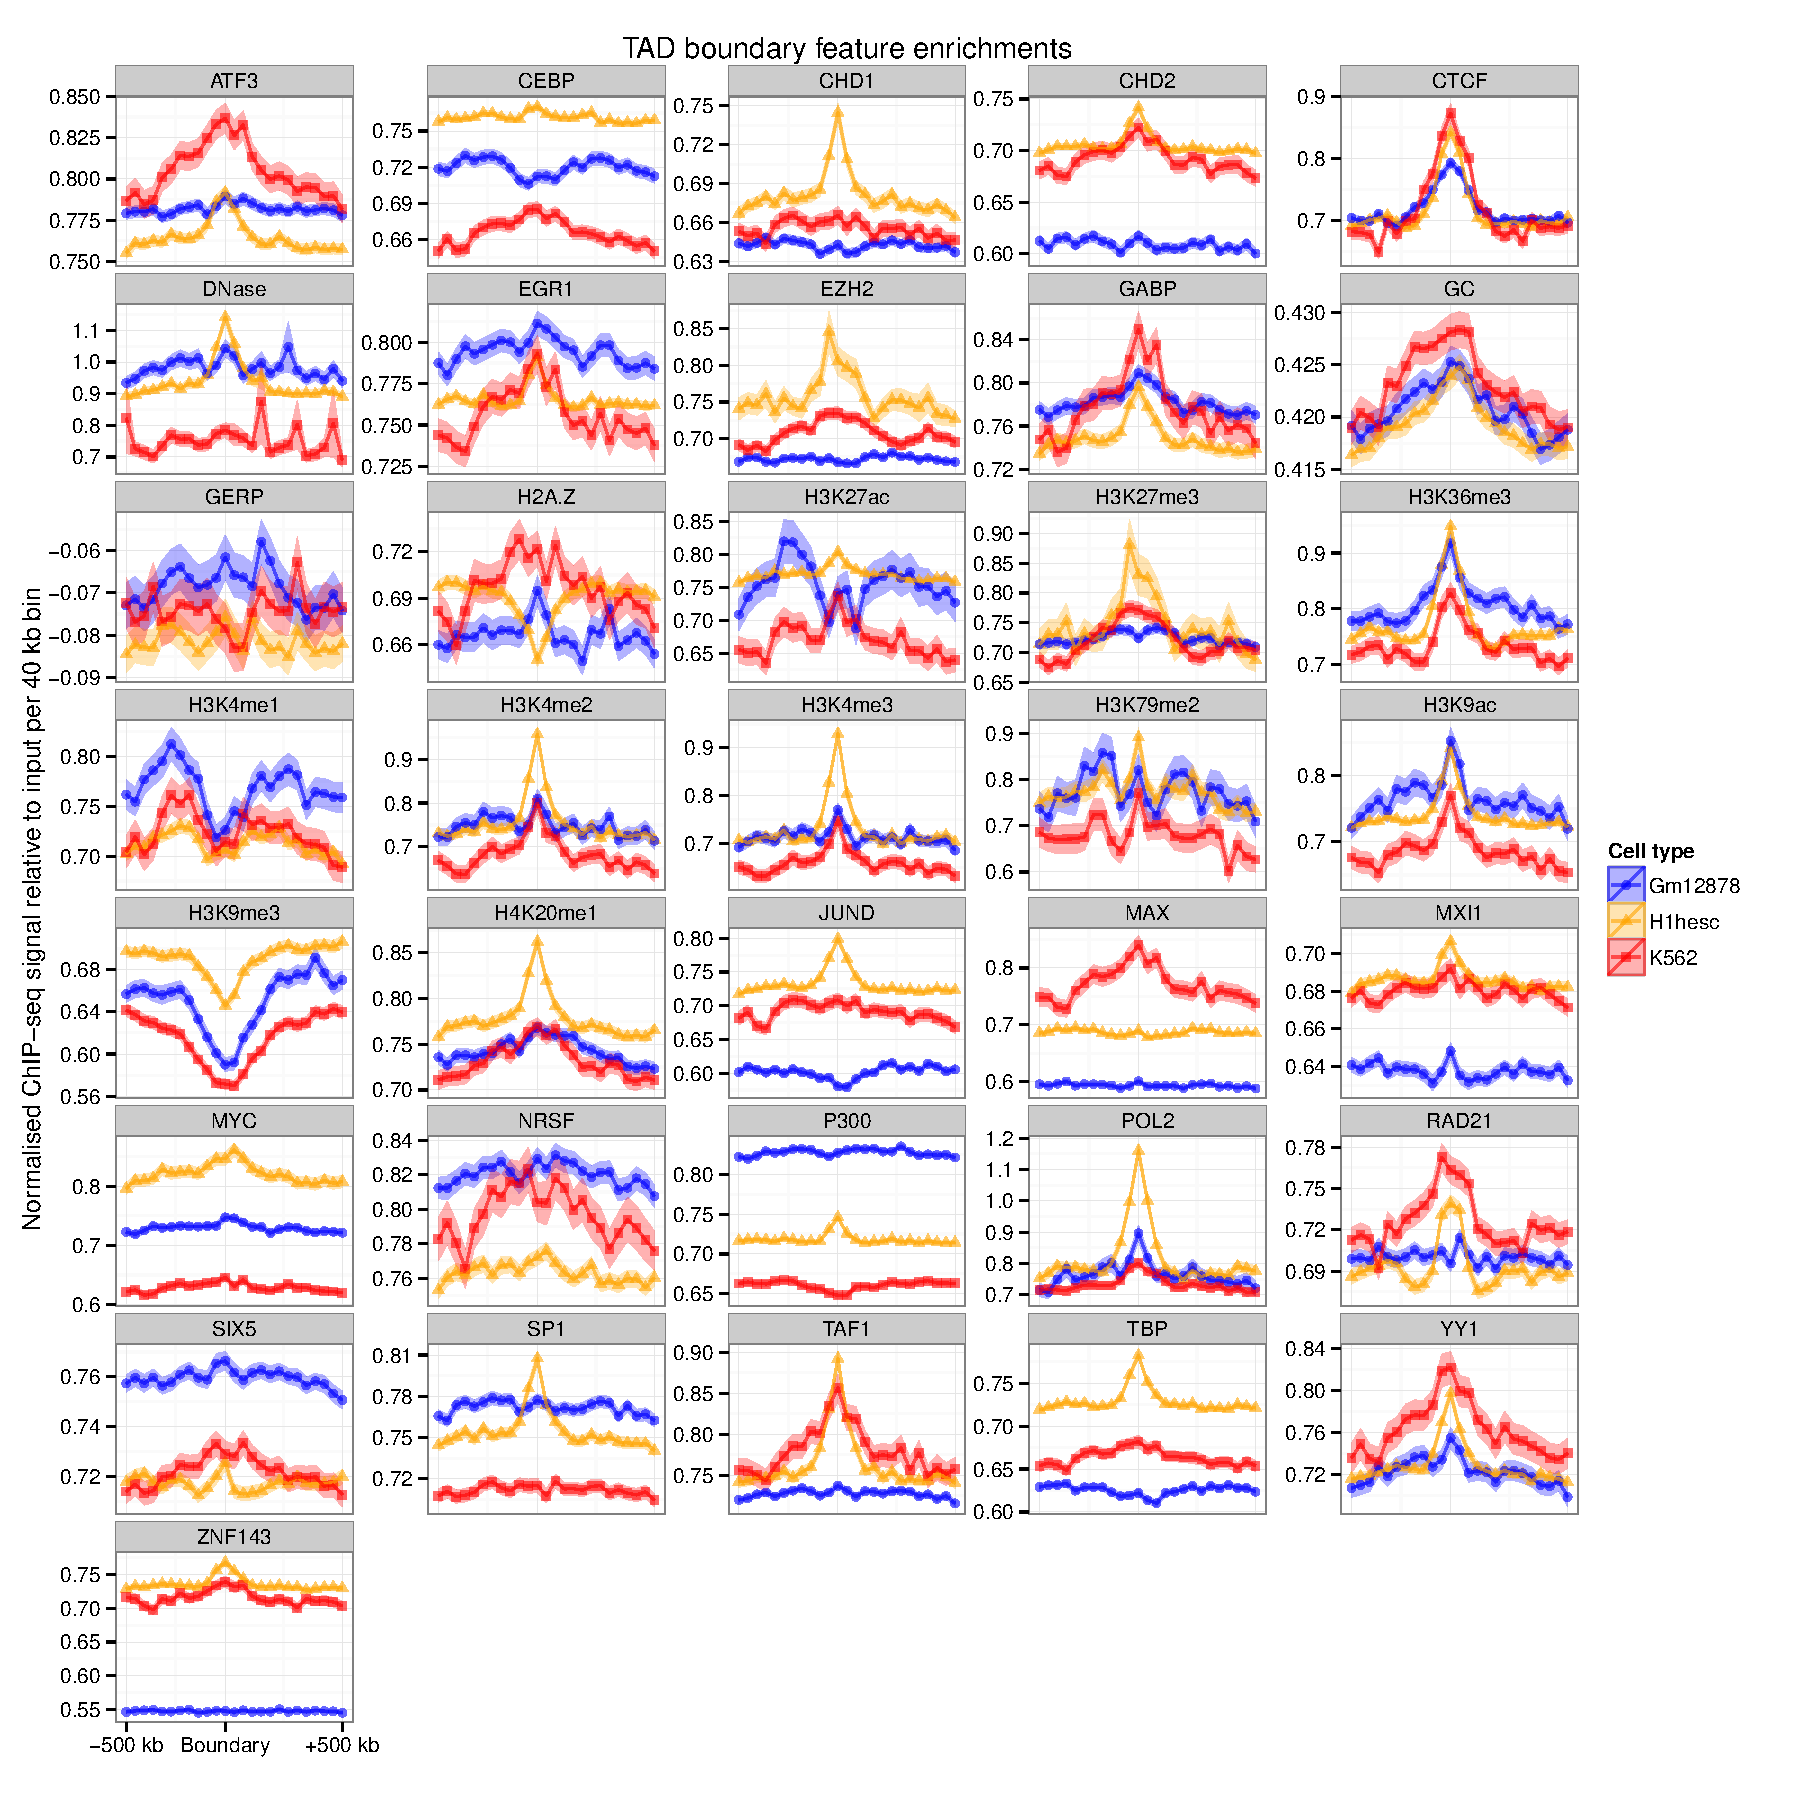
\includegraphics[width=6.8in]{alltads.pdf}
}
\captionsetup{width=\textwidth}
\caption[TAD boundary enrichments and depletions.]{ {\bf TAD boundary enrichments and depletions.}
36 features were averaged over 1 Mb windows centred on TAD boundaries genome-wide ($25 \times 40$ kb bins). Ribbons represent $95\%$ confidence intervals of the mean at each position.
}\label{fig:alltads}
\end{center}
\end{figure} 

Our findings confirmed the previously reported peaks (CTCF and POL2) and dip (H3K9me3) in ESC data, but also revealed substantial heterogeneity between cell types and some novel boundary features. CTCF binding was found enriched at TAD boundaries across all cell types, but other features, including H3K27me3 and H3K4me3, show dramatic peaks of enrichment in H1 hESC cells that are not seen consistently in other cell types (Fig. \ref{fig:alltads}). Although the dip in H3K9me3 at TAD boundaries is seen in all cell types, the extent of the depletion varies and is weakest in H1 hESC cells. We also note an apparent enrichment of H4K20me1 over TAD boundaries in H1 hESC cells, a modification previously implicated in chromatin compaction.\cite{Evertts2013} Finally we observe consistent increases in GC content at TAD boundaries, at a scale that is difficult to explain in terms of those much smaller GC-rich features such as binding motifs or CpG islands (Fig. \ref{fig:alltads}). The statistical significance of these enrichments and depletions is considered in Section \ref{sec:boundsignif}.

\subsection{Compartment boundaries}

Where neighbouring genomic regions occupy contrasting A and B nuclear
compartments, the disparity implies the presence of a boundary
region. We identified putative compartment boundaries using an
HMM to infer the state sequence of A/B compartments across the genome
based on observed principal component eigenvectors (Section \ref{sec:compcalls}). Analogously to the
TAD boundary analysis we then sought significant enrichments or
depletions in our set of chromatin features over these compartment boundaries.  

\begin{figure}
\begin{center} 
\makebox[\textwidth][c]{ 
	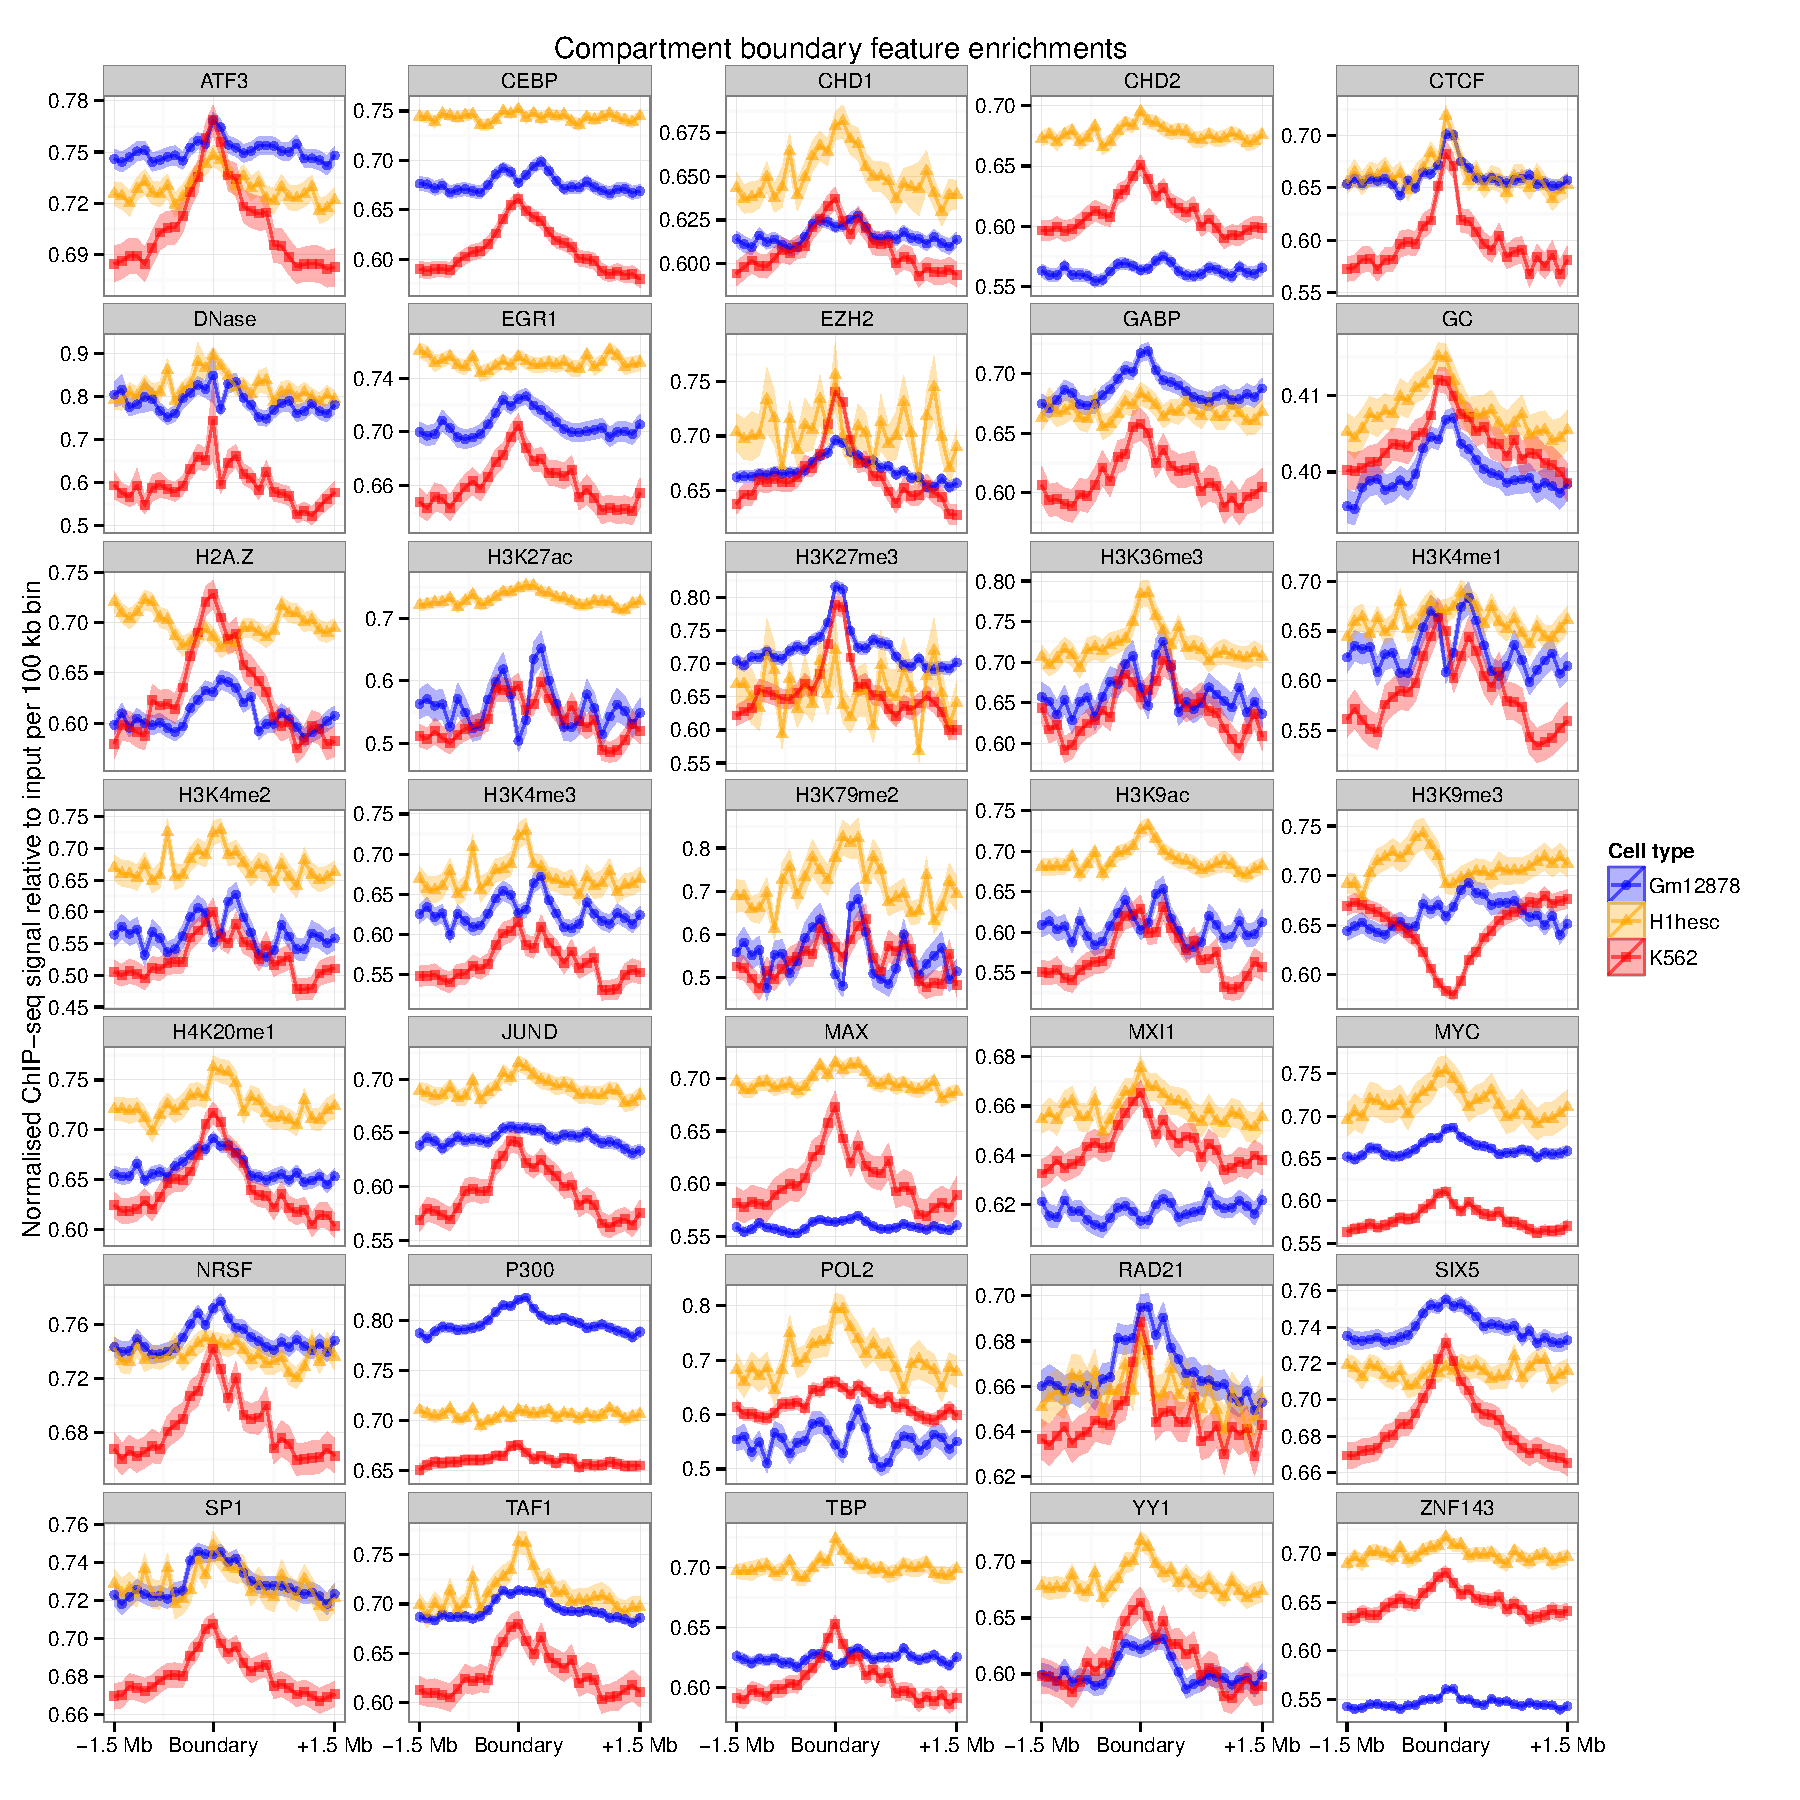
\includegraphics[width=6.8in]{allcompartments.pdf}
}
\captionsetup{width=\textwidth}
\caption[Compartment boundary enrichments and depletions.]{ {\bf Compartment boundary enrichments and depletions.}
36 features were averaged over 3 Mb windows centred on compartment boundaries genome-wide ($30 \times 100$ kb bins). Ribbons represent $95\%$ confidence intervals of the mean at each position.
}\label{fig:allcompartments}
\end{center}
\end{figure} 

Compartment boundaries display similar
spectra of enrichments to previously studied TAD boundaries
\cite{Dixon2012} but at lower resolution, reflecting the different
scales of these levels of organisation (Fig. \ref{fig:allcompartments}). 
Peaks associated with active promoters (POL2, TAF1, H3K9ac) are again
evident. Enrichments of CTCF and YY1 are again seen
at compartment boundaries, as they were for TAD boundaries, in each
cell type under study. In addition, compartment boundaries show
enrichments of H3K79me2, which is known to play a critical role in
cellular reprogramming.\cite{Onder2012} This histone modification has
also recently been shown to mark the borders of small (hundreds of bp)
regions of open chromatin,\cite{Chai2013} hinting at similarities in chromatin boundaries at very different scales.

Certain features show intriguing contrasts between cell types. For example, the
histone variant H2A.Z shows a clear enrichment over K562 compartment boundaries, but not the other two
cell types (Fig. \ref{fig:allcompartments}). Compartment
boundaries also show enrichment for the cohesin complex subunit RAD21
in the two hematopoietic cell types, and cohesin is
another factor implicated in modulating nuclear architecture in
partnership with CTCF.\cite{Zuin2013} Various other enrichments
of modest effect size can also be seen (Fig. \ref{fig:allcompartments}). In contrast with TAD boundaries, the
composition of compartment boundaries appears least complex in H1
hESC, relative to the other two cell types (cf. Fig. \ref{fig:allcompartments}). 

% new stuff here for thres Vs HMM boundaries
These enrichments over compartment boundaries offer the opportunity to investigate the effects of the HMM boundary calling method used in this work with the previously-used simple thresholding approach.\cite{Lieberman2009} To this end we compared that subset of boundaries retained through HMM calling (for details see Section \ref{sec:compcalls}), with those that would have been called through simple thresholding when the compartment eigenvector changes sign. We find that boundary enrichments are largely reduced or absent in this latter set of boundaries (Fig. \ref{fig:hmmVthres}). This result suggests that the HMM boundary calling method is filtering noisy compartment boundary calls which would otherwise be present through a simple thresholding approach, however we note that the absence of boundary enrichment does not necessarily preclude the presence of a compartment boundary.

\begin{figure}
\begin{center} 
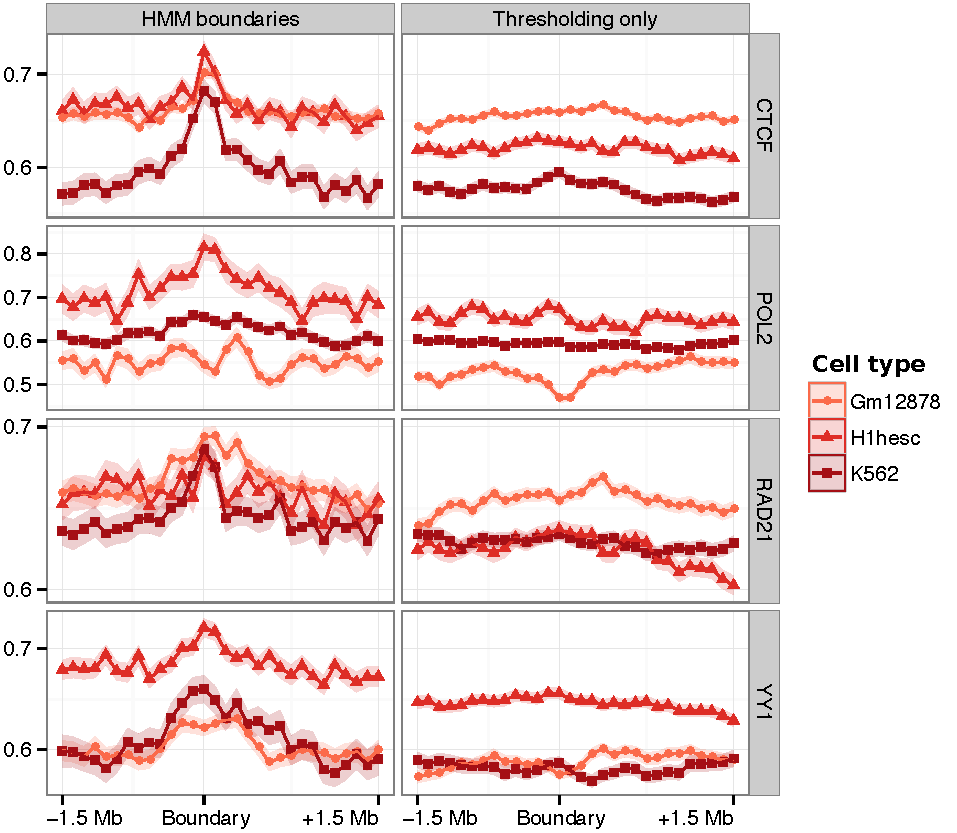
\includegraphics[width=3in]{hmmVthres.pdf}
\captionsetup{width=\textwidth}
\caption[ Compartment boundary candidates filtered through HMM calling show reduced feature enrichments. ]{ {\bf Compartment boundary candidates filtered through HMM calling show reduced feature enrichments. }
Boundary feature enrichments are compared for boundaries called via the HMM method described in this work (discussed in Section \ref{sec:compcalls}), and boundaries omitted through the HMM method but present if a simple thresholding approach is used to delimit compartment domains. Boundary profiles shown as in Figure \ref{fig:allcompartments}.
}\label{fig:hmmVthres}
\end{center}
\end{figure} 

\subsection{Significance testing of boundary associations}\label{sec:boundsignif}

Domain boundary associations with other chromatin features are most frequently presented through the statistics-free "average-o-grams" similar to those presented in this work (Figs. \ref{fig:alltads}, \ref{fig:allcompartments}). We then went on to perform a quantitative test of the associations between these features with compartment and TAD boundaries. In brief, we compare the values for each normalised signal directly over a boundary bin with those peripheral bins in each $\approx 1$ Mb window (for TADs). We then perform a non-parametric, rank-based significance test to look for statistically significant enriched or depletions of each feature. Details of this procedure are given in Methods \ref{meth:tadbounds}.

\begin{figure}
\begin{center} 
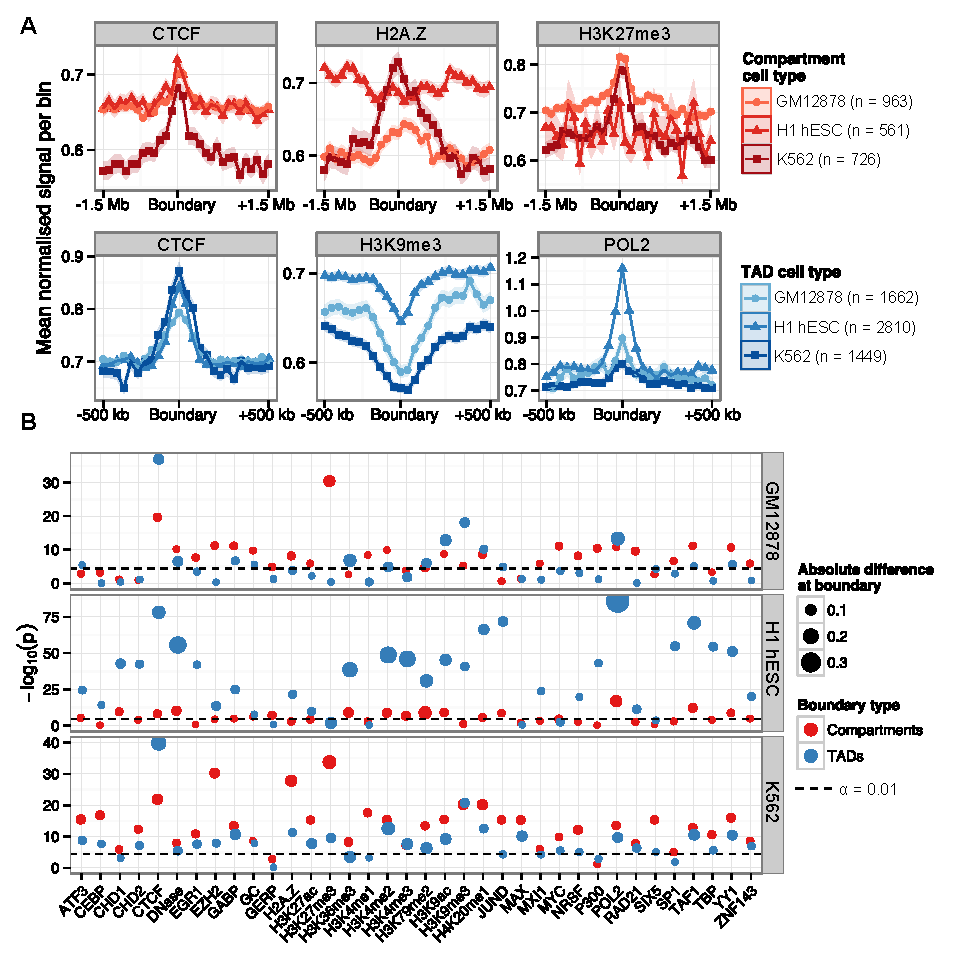
\includegraphics[width=5.5in]{boundarysummary.pdf}
\captionsetup{width=\textwidth}
\caption[Compartment and TAD boundary enrichment summary in three human cell types.]{ {\bf Compartment and TAD boundary enrichment summary in three human cell types.}
(A) Selected profiles for locus-level features are shown for compartment boundaries (CTCF, H2A.Z and H3K27me3) and TAD boundaries (CTCF, H3K9me3 and POL2), as a mean normalized ChIP-seq signal relative to input chromatin per bin ($\pm1$ standard error). TAD boundaries were examined over $40$ kb bins over the $1$ Mb flanking each boundary; compartment boundaries were examined in 100 kb bins over $3$ Mb. (B) The significance of enrichment or depletion ($-\log_{10}(p)$ two-tailed Mann--Whitney test) of a feature was calculated as the boundary bin relative to the ten most peripheral bins (five either side). Points are scaled by the absolute mean difference in signal over the boundary relative to the mean of peripheral bins.
}\label{fig:boundarysummary}
\end{center}
\end{figure} 

Results of this significance testing, along with selected boundary profiles, are presented in Figure \ref{fig:boundarysummary}. Overall we find that compartment and TAD boundaries are associated with overlapping spectra of highly significant enrichments and depletions of chromatin features across cell types. Across all tests (Fig. \ref{fig:boundarysummary}), we frequently find boundary enrichments for DNA binding proteins implicated in chromosome architecture (e.g. CTCF, YY1, RAD21), but also note broad enrichments for classes of input features associated with active transcription (e.g. POL2, TBP, H3K9ac). 

Reflecting their different scales, we find enrichment and depletion profiles typically
spanning regions of up to 500 kb for TAD boundaries but those over compartment boundaries often span more than a megabase (Fig. \ref{fig:boundarysummary}). We expect part of the reason for this discrepancy is the resolutions at which domains were called: TADS are resolved to 40 kb bins while compartment boundaries fall between megabase-sized bins. A further consideration is that larger numbers of TAD boundaries were called in the H1 hESC cell line, due its more deeply-sequenced Hi-C library (Section \ref{sec:calledtads}), giving greater statistical power to detect enrichments thus resulting in smaller $p$-values (Fig. \ref{fig:boundarysummary}). The lower resolution megabase bins used in compartment calling do not suffer from this issue.

%Altogether a large number of features show significant, though often modest, association with TAD and/or compartment boundaries. In terms of overall complexity boundaries (measured as the number of strongly enriched features) is notably higher in H1 hESC than in the other two, more differentiated, cell types (Fig. \ref{fig:boundarysummary}), involving large increases in the binding of sequence specific factors such as SP1 and JUND.


\subsection{CTCF and YY1}\label{sec:ctcfyy1}

\begin{figure}
\begin{center} 
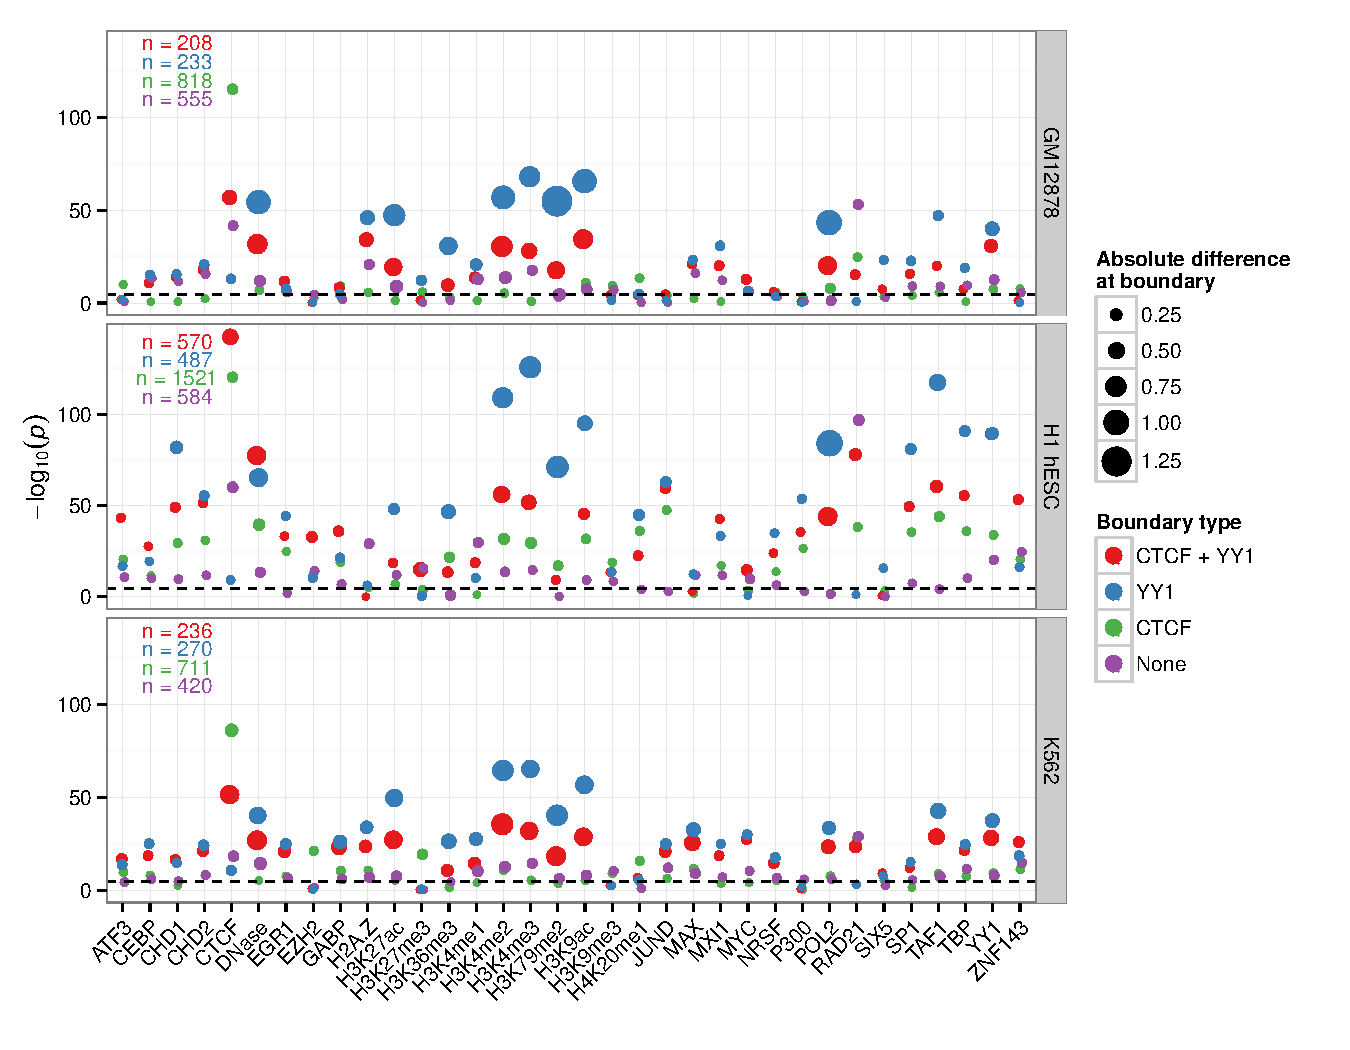
\includegraphics[width=5.8in]{ctcfyy1.pdf}
\captionsetup{width=\textwidth}
\caption[Distinct enrichments of CTCF and YY1 boundaries.]{ {\bf Distinct enrichments of CTCF and YY1 boundaries.}
The significance of TAD boundary enrichments and depletions are shown (as in Fig. \ref{fig:boundarysummary}) for boundaries
split into classes based on the presence or absence of ChIP-seq peaks within boundary bins. CTCF and YY1 groups are
those boundaries with at least one ENCODE region peak\cite{Dunham2012} for
their respective features, while CTCF + YY1 is the group of boundaries which had one or more
overlapping peaks for these two factors. Boundaries in the "none" group had neither
a CTCF or YY1 region peak called (but can still
be enriched for their respective features in terms of raw signal). 
}\label{fig:ctcfyy1}
\end{center}
\end{figure} 

Significant boundary enrichments for both CTCF and YY1 are evident in all cell
types at both compartment and TAD boundaries (Fig. \ref{fig:boundarysummary}), which is intriguing given the evidence that YY1 and CTCF
cooperate to affect long distance interactions.\cite{Atchison2014} Co-binding of CTCF with YY1 has also been shown
to identify a subset of highly conserved CTCF sites.\cite{Schwalie2013} This colocation may also therefore be
a contributing factor in the establishment of TAD boundaries, which
appear to be broadly conserved across mammals.\cite{Dixon2012} 

To test this, we split our sets of TAD boundaries into those possessing
ChiP-seq peaks (region peaks as called by the ENCODE data processing pipeline\cite{Dunham2012}) for
CTCF, YY1, both CTCF and YY1 (overlapping peaks) and neither. We then
tested each boundary subset for genome-wide enrichments of the other
features in our dataset (Fig. \ref{fig:ctcfyy1}). Unexpectedly, we found that those
boundaries marked by YY1 but without overlapping CTCF peaks were
generally most strongly-enriched for other features in our dataset. This result potentially highlights YY1 as an under-appreciated contributor to boundary demarcation, particularly relative to the well-studied CTCF. We
also found that boundaries lacking both CTCF and YY1 peaks showed
instead the strongest enrichments for RAD21 in each cell type (Fig. \ref{fig:ctcfyy1}), reinforcing previous findings that describe the distinct
influences of CTCF and cohesin in organising chromatin structure.\cite{Zuin2013, Seitan2013, Phillips-Cremins2013}

% Schwalie: These observations suggest that with respect to transcriptional activity, YY1 is the functionally dominant factor at co-bound locations.

\subsection{Repeats}\label{sec:repeats}

\citet{Dixon2012} identified short interspersed element (SINE) repeats as being enriched over TAD boundaries and suggested roles for these repeats in altering genome organisation, in line with prior evidence.\cite{Dixon2012, Lunyak2007} For example, SINE elements are thought to be responsible for spreading CTCF binding sites through mammalian genomes during evolution.\cite{Schmidt2012}  Analysis of recent high-resolution Hi-C data again reported a SINE B2 link with CTCF loops in mice,\cite{Rao2014} and examples have been reported of human genes whose expression has been altered by CTCF sites inserted through Alu repeats.\cite{Ruiz-Narvaez2008} Together these results suggest repeats could be a key component in the makeup of domain boundaries.

To investigate this, we used the \texttt{RepeatMasker}\cite{Tarailo-Graovac2009} software package to call repeat classes and families in the \texttt{hg19} and \texttt{mm10} genome assemblies. Counts for each annotated feature were then averaged over boundaries as described previously (Methods \ref{boundaries}).

\begin{figure}
\begin{center} 
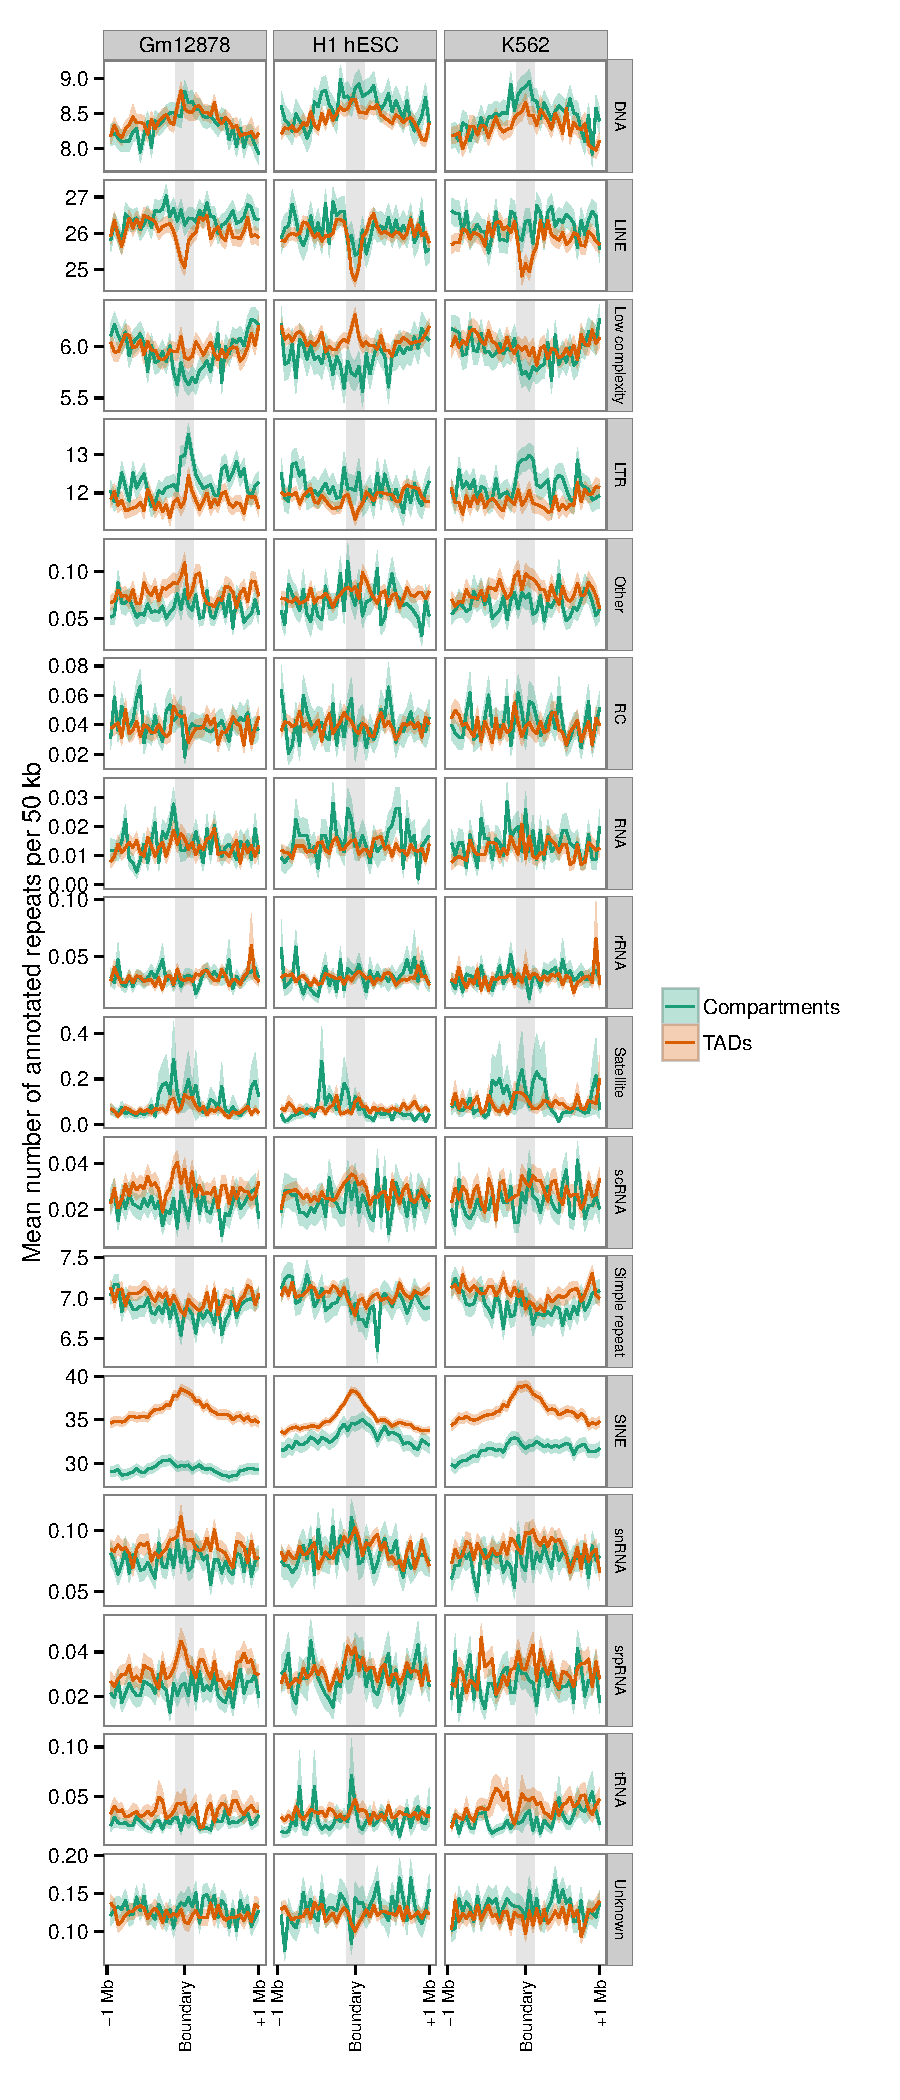
\includegraphics[width=3.95in]{rep_classprofiles.pdf}
\captionsetup{width=\textwidth}
\caption[Repeat class average-o-grams over all TAD and compartment boundaries.]{ {\bf Repeat class average-o-grams over all TAD and compartment boundaries.}
\texttt{RepeatMasker} repeat annotations are counted per 50 kb for 1 Mb either side of all TAD and compartment boundaries. The mean counts per bin genome-wide are plotted with $\pm 95\%$ confidence intervals.
}\label{fig:rep_classprofiles}
\end{center}
\end{figure} 

At the level of repeat class, we corroborate the findings of \citet{Dixon2012} that the majority of repeat classes show no enrichment or depletion at TAD boundaries, and we find that this also holds for compartment boundaries (Fig. \ref{fig:rep_classprofiles}). A notable exception is the short interspersed element (SINE) repeat class which appears to be enriched at TAD boundaries in each cell type. Testing the significance of this observed peak confirms this to be the case, with SINEs significantly enriched at TAD boundaries in each cell type, and borderline significant enrichments can also be observed at compartment boundaries (Fig. \ref{fig:rep_classbubble}).

\begin{figure}
\begin{center} 
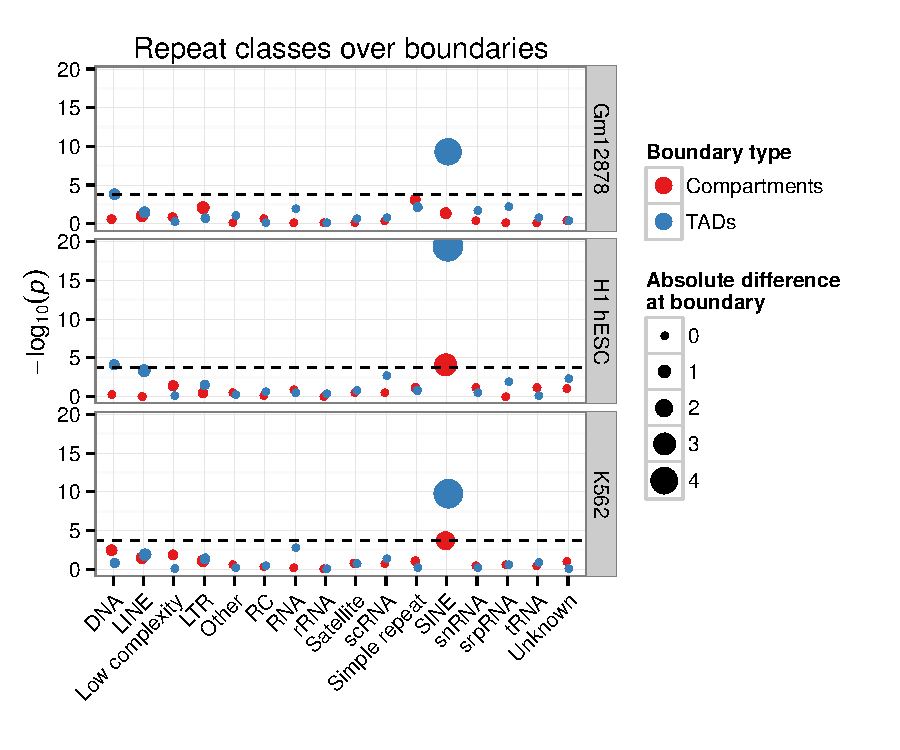
\includegraphics[width=3.2in]{rep_classbubble.pdf}
\captionsetup{width=\textwidth}
\caption[Significance and effect sizes of repeat class enrichments and depletions over boundaries.]{ {\bf Significance and effect sizes of repeat class enrichments and depletions over boundaries.}
Boundary profiles (as shown in Figure \ref{fig:rep_classprofiles}) were each tested for enrichment or depletion of each repeat class at the boundary bin relative to peripheral non-boundary bins (see Methods \ref{boundaries}). Bubble area is proportional to the raw effect size of an enrichment or depletion. The Bonferroni-corrected significance threshold is highlighted with a dashed line.
}\label{fig:rep_classbubble}
\end{center}
\end{figure} 

We also find long interspersed elements (LINEs) are significantly depleted over TAD boundaries in two cell types, and borderline significant in the third, though with modest effect sizes in each case (Figs. \ref{fig:rep_classprofiles}, \ref{fig:rep_classbubble}). DNA repeats appear to be enriched at both boundary types (Fig. \ref{fig:rep_classprofiles}), however these observations do not surpass our significance threshold ($\alpha = 0.05$) after multiple testing correction (Fig. \ref{fig:rep_classbubble}).

Repeat classes can be broken into smaller repeat families. \citet{Dixon2012} reported that the Alu repeat family of the SINE repeat class (or SINE B2 in mouse) is enriched over TAD boundaries. Again we can reproduce this finding and extend the analysis to compartment boundaries, where we do not see a significant enrichment for Alu repeat elements (Fig. \ref{fig:rep_fambubble}). Surprisingly almost all other repeat families show no significant departure from their expected levels over TAD or compartment boundaries. 
%In contrast with the Alu family of SINEs, no individual LINE element family displays significant depletions at TAD boundaries (Fig. \ref{fig:rep_fambubble}), consistent with the action of purifying selection to remove these much larger insertions in boundary regions. However, mysteriously no other significant depletions are seen for large insertions originating from other repeat families e.g. ERV-related families.

\begin{figure}
\begin{center} 
\makebox[\textwidth][c]{ 
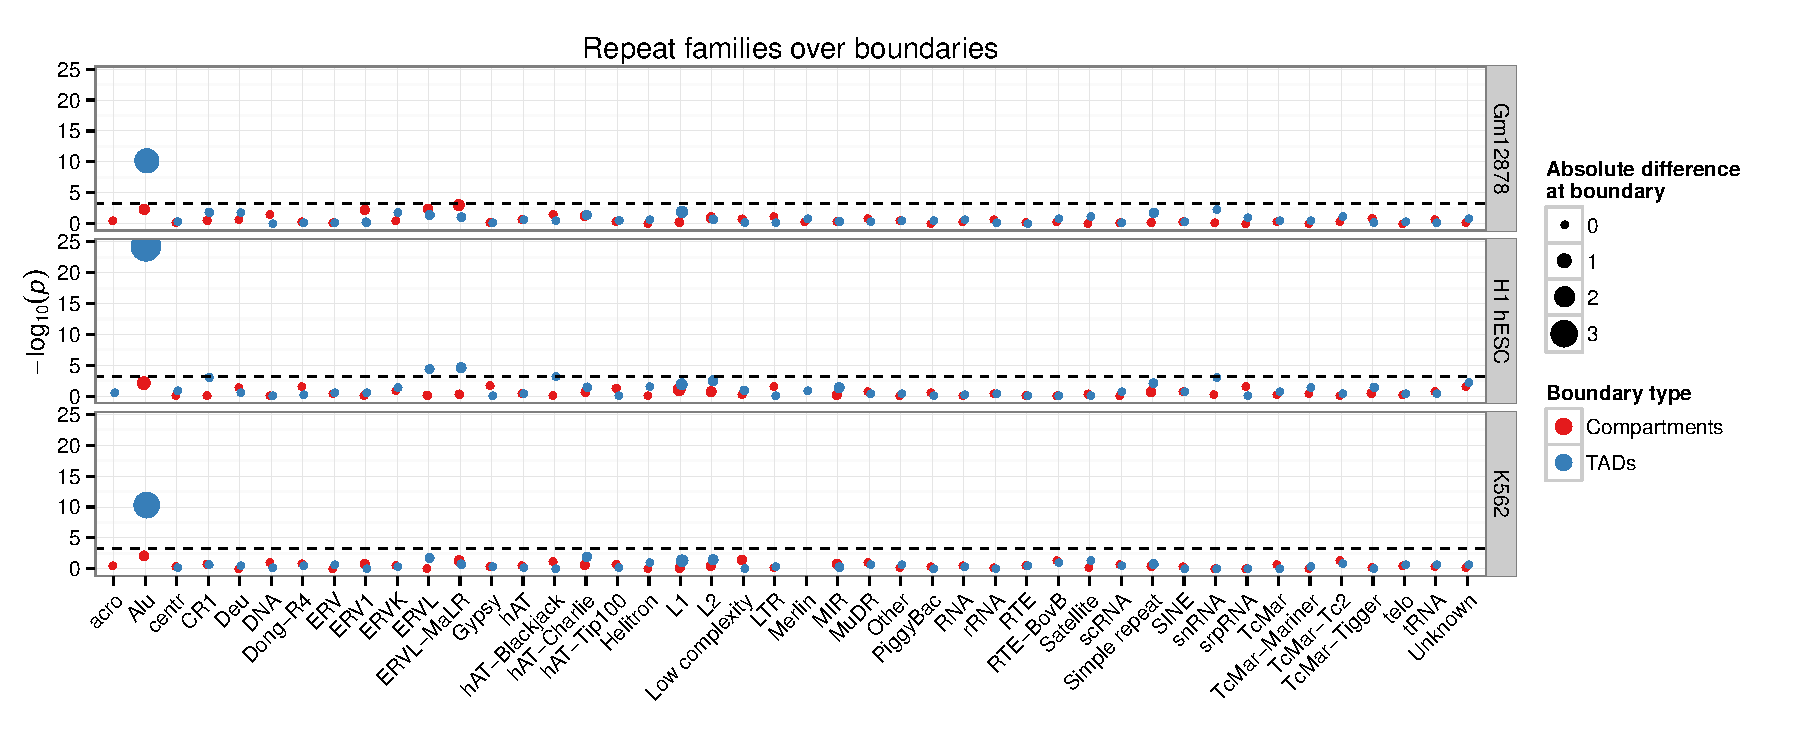
\includegraphics[width=7in]{rep_fambubble.pdf}
}
\captionsetup{width=\textwidth}
\caption[Significance and effect sizes of repeat family enrichments and depletions over boundaries.]{ {\bf Significance and effect sizes of repeat family enrichments and depletions over boundaries.}
As per Figure \ref{fig:rep_classbubble} but for a more specific repeat classification.
}\label{fig:rep_fambubble}
\end{center}
\end{figure} 

% Figure: profiles of those significant + suggestive from all repeat family profiles

\section{TAD boundary prediction}\label{sec:boundarypred}

We have shown TAD and compartment domain boundaries to be reliably and significantly marked by a variety of features. Compartment boundaries are successfully predicted as a side-effect of modelling the continuous compartment profile eigenvector (Section \ref{sec:modhoc}), reflecting global patterns of transcriptional activation and repression, however a related measure of activity and repression, or other comparable profile we might want to predict, does not exist for TADs. Instead then, in this section we attempt to predict TAD boundaries within a class-balanced classification framework.

%We attempted to model TAD boundaries in a variety of ways: firstly a using a class-balanced classification framework and secondly through indirect models of directionality index and the downstream domain-caller HMM state.\cite{Dixon2012}

\subsection{Learning boundary classification}\label{sec:tadpred}

Results presented in this thesis describe the spectra of chromatin marks over TAD boundaries (Figs. \ref{fig:alltads}, \ref{fig:boundarysummary}), thus it is of interested to test if we can build a predictive model (in the manner of Chapter \ref{chap:modelling}) that can call boundary regions from these marks alone. Such a model, if successful, could have broad utility in domain prediction in metazoan organisms where Hi-C data is not available.

A straightforward approach to this modelling task is to build a supervised classifier that learns the associations between two classes of genomic region: those labelled TAD boundaries and those which are not. To this end, we again turn to a Random Forest (RF) model, due to its many attractive properties discussed previously (Methods \ref{sec:rf}). Our input feature set is made up of the same $35$ matched features used in models of compartment eigenvector (Section \ref{sec:modhoc}), with the addition of Alu repeat element counts (Section \ref{sec:repeats}). Domain calls are those produced by the \citet{Dixon2012} TAD calling algorithm (Methods \ref{meth:tadcalling}), therefore TAD boundaries were resolved to 40 kb bins. We class TAD boundary bins as boundary true positives (TP), and select matched bins $500$ kb upstream as boundary true negatives (TN) for our training set.

To build parsimonious and accurate models (as discussed in Section \ref{sec:parsimoniousmodels}), we used the \texttt{AUC-RF} algorithm.\cite{Calle2011} This is a form of stepwise model selection which optimises feature subset selection relative to the area under the receiver operating characteristic (AUROC), a metric which captures both the specificity and sensitivity of a classifier. The AUC-RF algorithm was applied to a training set of $80\%$ of boundaries per cell type, with predictions assessed on out-of-bag (OOB) data as each forest was constructed. Selected models were then applied to the remaining held-out test set of $20\%$ of TAD boundaries, with their matched non-boundary bins (full details are given in Methods~\ref{meth:tadpred}). 

% AUC-RF optimisation plots
%        AUC  k      ct
%1 0.6636421 26 GM12878
%2 0.7086773 17 H1 hESC
%3 0.6645574 15    K562
\begin{figure}
\begin{center} 
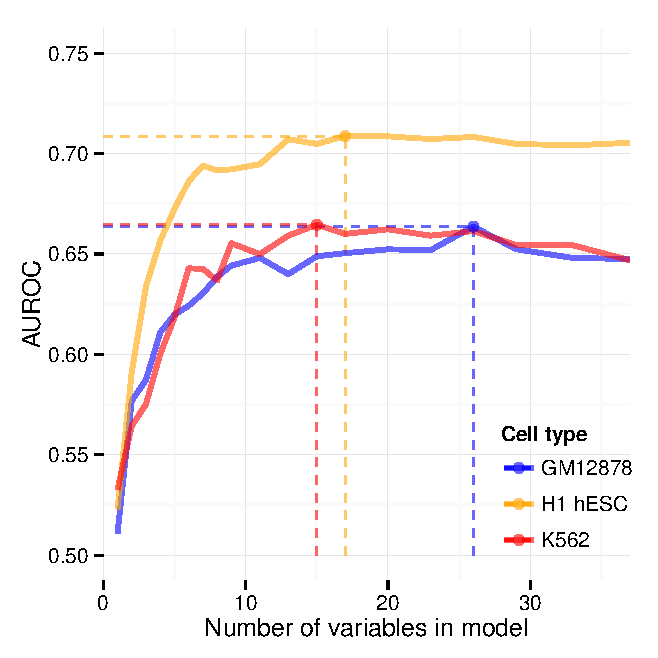
\includegraphics[width=3in]{AUCRF_opt.pdf}
\captionsetup{width=\textwidth}
\caption[ The AUC-RF stepwise algorithm finds that variable subset which maximises the AUROC on out-of-bag data. ]{ {\bf The AUC-RF stepwise algorithm finds that variable subset which maximises the AUROC on out-of-bag data. }
The AUROC is calculated at each stage of a stepwise method for selecting the best subset model from a full featureset. Here AUC-RF selected the following combinations: GM12878: 26 vars, 0.66 AUC; H1 hESC: 17 vars, 0.71 AUC; K562: 15 vars, 0.66 AUC. The AUC-RF algorithm is described in Methods \ref{meth:tadpred}.
}\label{fig:tadpred_opt}
\end{center}
\end{figure} 


Predictive performance of these models is shown as ROC plots (Fig. \ref{fig:tadpred_auroc}) and in each case an AUROC of around $0.67$--$0.71$ was achieved. In practice, this means that each classifier has around a $70\%$ probability of ranking a random boundary region more highly than a random non-boundary region.\cite{Fawcett2006a} According to a commonly-used AUROC rule of thumb, this performance falls between the ranges of "poor" to "moderate" classification accuracy.\cite{Streiner2007a}

\begin{figure}
\begin{center} 
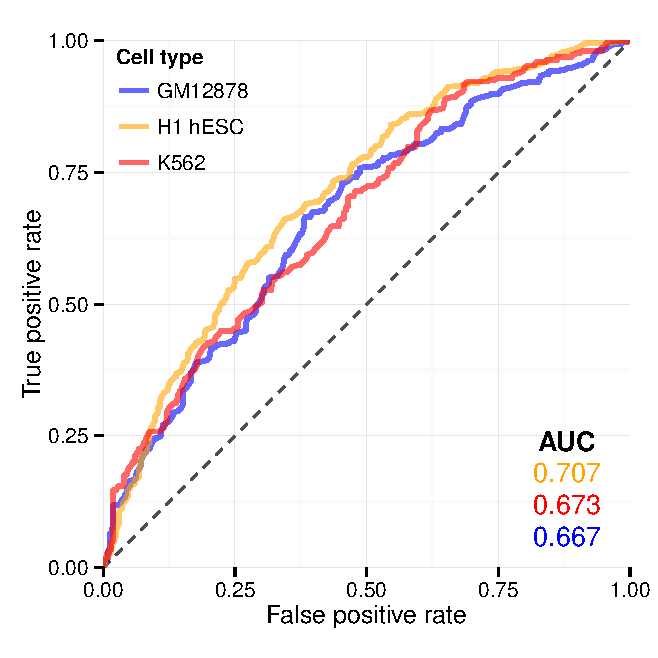
\includegraphics[width=3in]{tadpred_auroc.pdf}
\captionsetup{width=\textwidth}
\caption[ Receiver operating characteristics for TAD boundary classifications. ]{ {\bf Receiver operating characteristics for TAD boundary classifications. }
ROCs are shown for three cell type specific classifiers of TAD boundary bins. The area under each cure is also shown (\emph{inset}).
}\label{fig:tadpred_auroc}
\end{center}
\end{figure} 

Despite this sub-optimal classification accuracy, it is still of interest to analyse the variable importances in each cell type model. Strikingly we find that CTCF stands out as the most informative variable in each classifier by some margin (Fig. \ref{fig:tadpred_varimp}). This is in agreement with our results that CTCF showed among the highest and most consistent enrichments at TAD boundaries (Fig. \ref{fig:boundarysummary}). RAD21 is also highly ranked in each case and this ties in with our previous results suggesting orthogonal boundary enrichments for either CTCF or RAD21 (Section \ref{sec:ctcfyy1}). Surprisingly YY1 does not feature as highly ranked in any model despite our observed consistent enrichments at TAD boundaries (Fig. \ref{fig:boundarysummary}). In fact YY1 was pruned from the optimal H1 hESC and GM12878 models by the AUC-RF algorithm due to its low variable importance (\emph{data not shown}). This could be due to a redundancy between information provided by YY1 and the CTCF variable as, for example, co-binding of YY1 and CTCF is thought to occur at sites of long-range chromatin interactions.\cite{Atchison2014} 

\begin{figure}
\begin{center} 
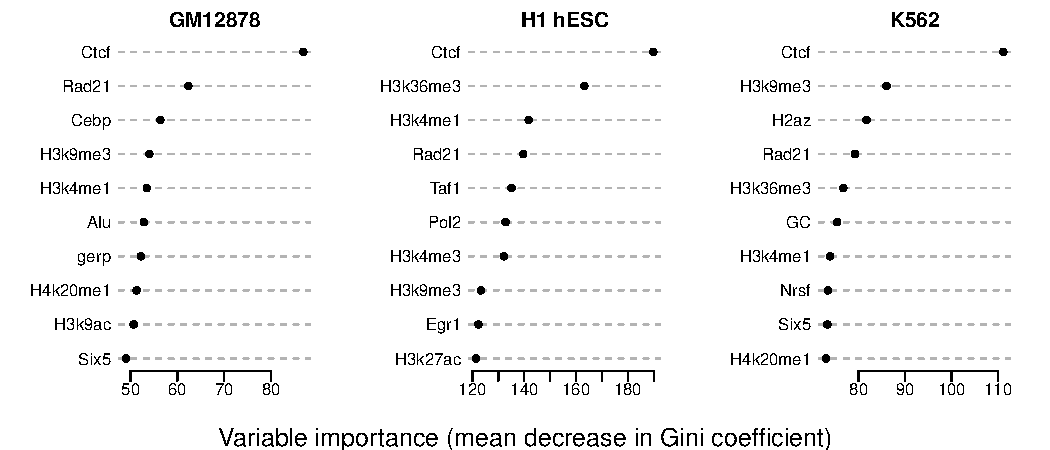
\includegraphics[width=5.45in]{tadpred_varimp.pdf}
\captionsetup{width=\textwidth}
\caption[ Variable importance for boundary classification Random Forest models. ]{ {\bf Variable importance for boundary classification Random Forest models. }
The ten most important variables in each boundary classification model are shown and ranked by their variable importance as defined by mean decrease in Gini impurity (Methods \ref{meth:gini}).
}\label{fig:tadpred_varimp}
\end{center}
\end{figure} 

%\subsection{Modelling performance}
% 
%The modelling performance achieved above with TAD boundaries (Fig. \ref{fig:tadpred_auroc}) is notably lower than previous models of transcription and compartment eigenvectors (Chapter \ref{chap:modelling}).

\section{MetaTAD boundaries}\label{sec:metatads}

Our collaborators in the Pombo lab (Max Delbr\"{u}ck Center, Berlin) proposed the concept of "metaTADs": sequential aggregations of adjacent and strongly-interacting TADs that form a hierarchy of domain organisation covering each chromosome.

MetaTADs are constructed simply by performing constrained hierarchical clustering based on inter-domain contacts. That is, those two neighbour TADs that have the largest number of inter-TAD contacts are linked to form a metaTAD and this process is recursed until all TADs on a chromosome are joined into a single tree which fully describes the hierarchical nature of domain organisation (\emph{manuscript under revision}).

My contribution to this work was to explore these newly-described metaTAD structures and perform boundary analysis as was done with TADs and compartments (Section \ref{sec:boundaryenrichments}). A testable hypothesis, for example, is that boundaries of larger metaTAD structures could display greater enrichments for boundary-defining features.

\subsection{MetaTAD boundary comparison}\label{sec:metaVtad}

Due to the manner in which metaTADs were constructed by our collaborators, by sequential aggregation of TADs (Methods \ref{meth:meta}), boundary comparisons between TADs and metaTADs are not completely straightforward. Every metaTAD boundary is, at a lower level, also a TAD boundary hence for a meaningful comparison we compared only a subset of metaTAD boundaries. Selection of this threshold involved a trade-off between maintaining a sufficient sample size of metaTADs and minimising the overlap between metaTAD and TAD boundaries to increase the discriminative power of our comparison (Fig. \ref{fig:mtcalibrate}).

\begin{figure}
\begin{center} 
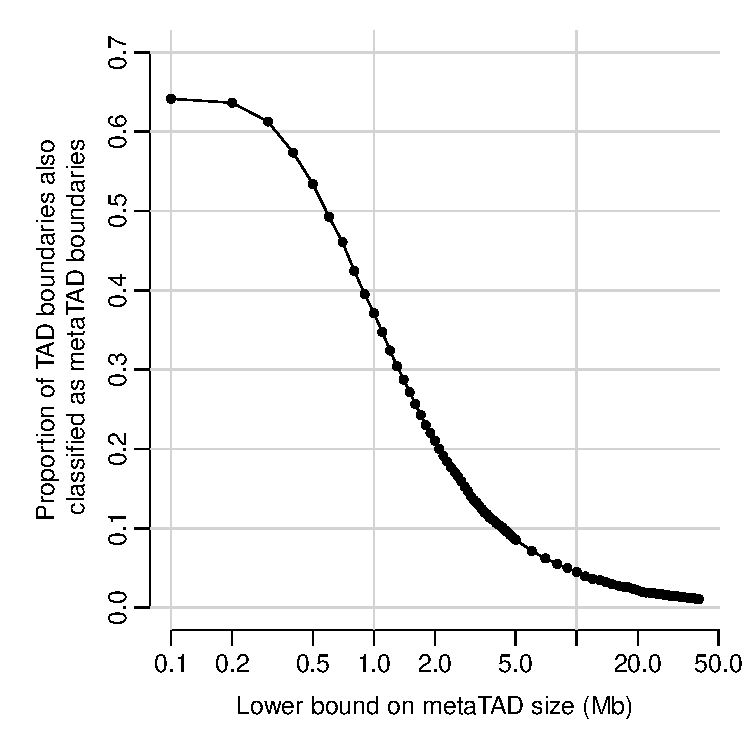
\includegraphics[width=2.75in]{mt_calibrate.pdf}
\captionsetup{width=\textwidth}
\caption[Calibration of metaTAD size selection bounds.]{ {\bf Calibration of metaTAD size selection bounds. }
As the lower bound on metaTAD size is increased, the proportion of all TAD boundaries which are also metaTAD boundaries decreases.
}\label{fig:mtcalibrate}
\end{center}
\end{figure} 

From the calibration plot (Fig. \ref{fig:mtcalibrate}), a lower bound metaTAD size cut-off of 10 Mb was selected for comparison with TAD boundaries. This left a reasonable sample size of $263$ metaTAD boundaries, while reducing the overlap with the set of all TAD boundaries to approximately $5\%$ (Fig. \ref{fig:mtcalibrate}). We also used an upper bound for size selection, based on observations by our collaborators that interactions between metaTADs larger than around $40$ Mb were no higher than expected background signal (\emph{data not shown}). In practice, almost all boundaries making up metaTADs larger than $10$ Mb are also present in those larger than $40$ Mb, but as hierarchical clustering continued up to the whole chromosome level, this upper bound may exclude a small number of edge-case peripheral TADs which aggregated into chromosome-wide metaTADs without evidence of heightened intra-TAD interactions.

Next a comparison between metaTAD boundaries for metaTAD size ($s$) in the range $10~\textrm{Mb} < s < 40~\textrm{Mb}$ was performed. Our collaborators generated several ChIP-seq datasets, including for CTCF and three PolII variants, as well as expression data in the form of CAGE (Methods \ref{meth:metadata}). We calculated the average profiles of each of these features over regions surrounding the set of all metaTAD and TAD boundaries (Fig. \ref{fig:mtfeats}). These average profiles show heightened enrichment for PolII variants, CTCF and DNase, with non-overlapping $95\%$ confidence intervals of the mean over the boundary bin. Profiles also suggest increased enrichments of gene density and the histone modification H3K27me3 at metaTAD boundaries relative to TAD boundaries (Fig. \ref{fig:mtfeats}). The co-incidence of metaTAD boundaries and lamina associated domains (LADs) is explored further in Section \ref{sec:mtlads}.

\begin{figure}
\begin{center} 
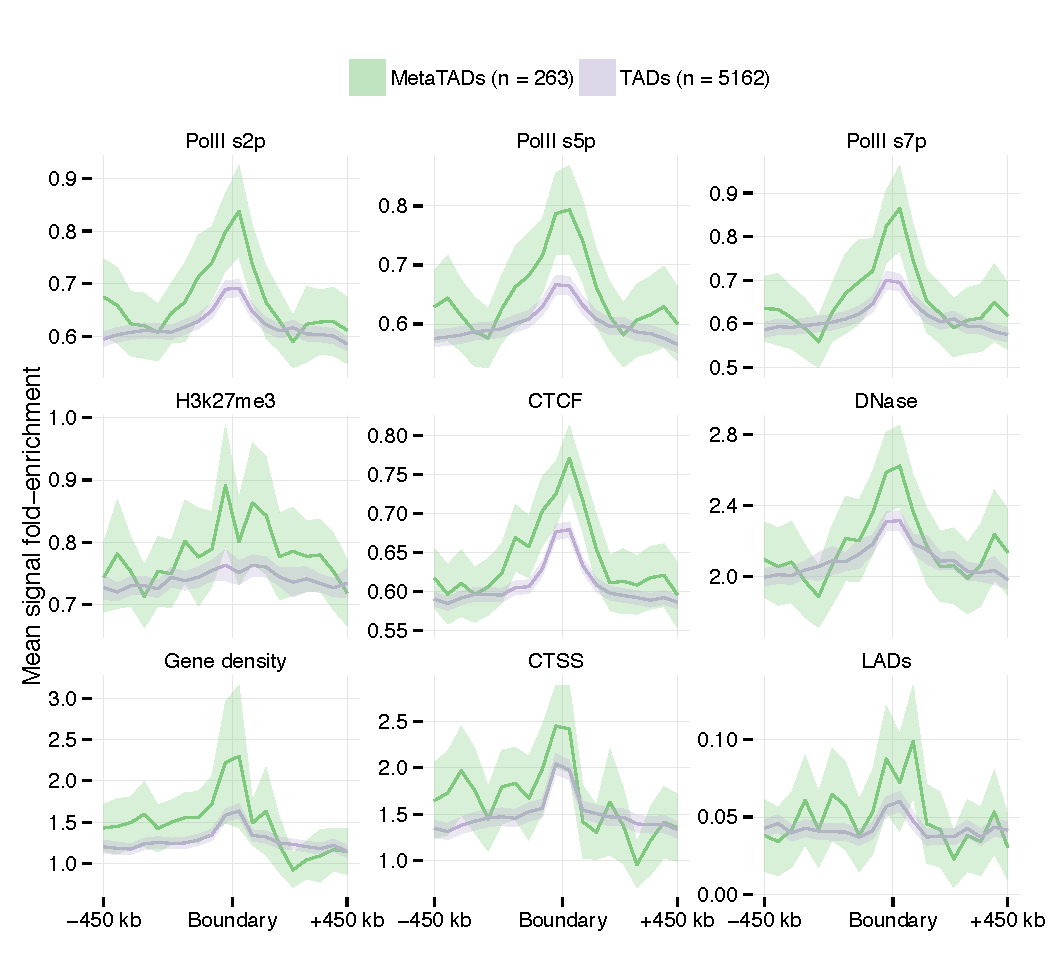
\includegraphics[width=4.5in]{mt_feats.pdf}
\captionsetup{width=\textwidth}
\caption[Large metaTADs show greater enrichments than TADs for an array of boundary features.]{ {\bf Large metaTADs show greater enrichments than TADs for an array of boundary features.}
Genome-wide profiles of epigenomic features and gene densities averaged over all TAD and metaTAD (10 -- 40 Mb) boundaries (ribbons show $95\%$ confidence intervals of the mean).
}\label{fig:mtfeats}
\end{center}
\end{figure} 

Increased enrichment at metaTAD boundaries relative to TAD boundaries lends evidence to the functional importance of metaTADs, and suggests boundaries become increasingly well-demarcated at higher levels of organisation. However, if this is a genuine biological phenomenon, we may expect the trend not just to be observable in a comparison between two selected sets, but to increase monotonically as we ascended the metaTAD hierarchy from TADs to chromosomes.

To test this, we reran the metaTAD boundary analysis (Fig. \ref{fig:mtfeats}) but at a range of metaTAD size cut-offs. Results of this analysis are shown in Figure \ref{fig:mtcutoffenrich}. Generally we find increasing enrichments in metaTAD boundaries relative to TAD bounds through the range of lower bound cutoffs from $0$ to $20$ Mb, possibly with a slight decreased effect size at the highest cutoff of $30$ Mb, where the sample size of boundaries decreases to just $62$ (Fig. \ref{fig:mtcutoffenrich}). This analysis strengthens the evidence for heightened functional enrichment of metaTAD boundaries (Figs. \ref{fig:mtfeats}, \ref{fig:mtcutoffenrich}) and suggests the metaTAD aggregation procedure is capturing boundaries of increasing strength, in terms of enrichment of boundary associated features, through the metaTAD hierarchy. Though the nature and significance of these boundary enrichments are currently open to debate, there exist precedents where greater enrichments over boundaries have been invoked as evidence that a novel TAD calling algorithm outperforms previous efforts.\cite{Filippova2014, Weinreb2015}

\begin{figure}
\begin{center} 
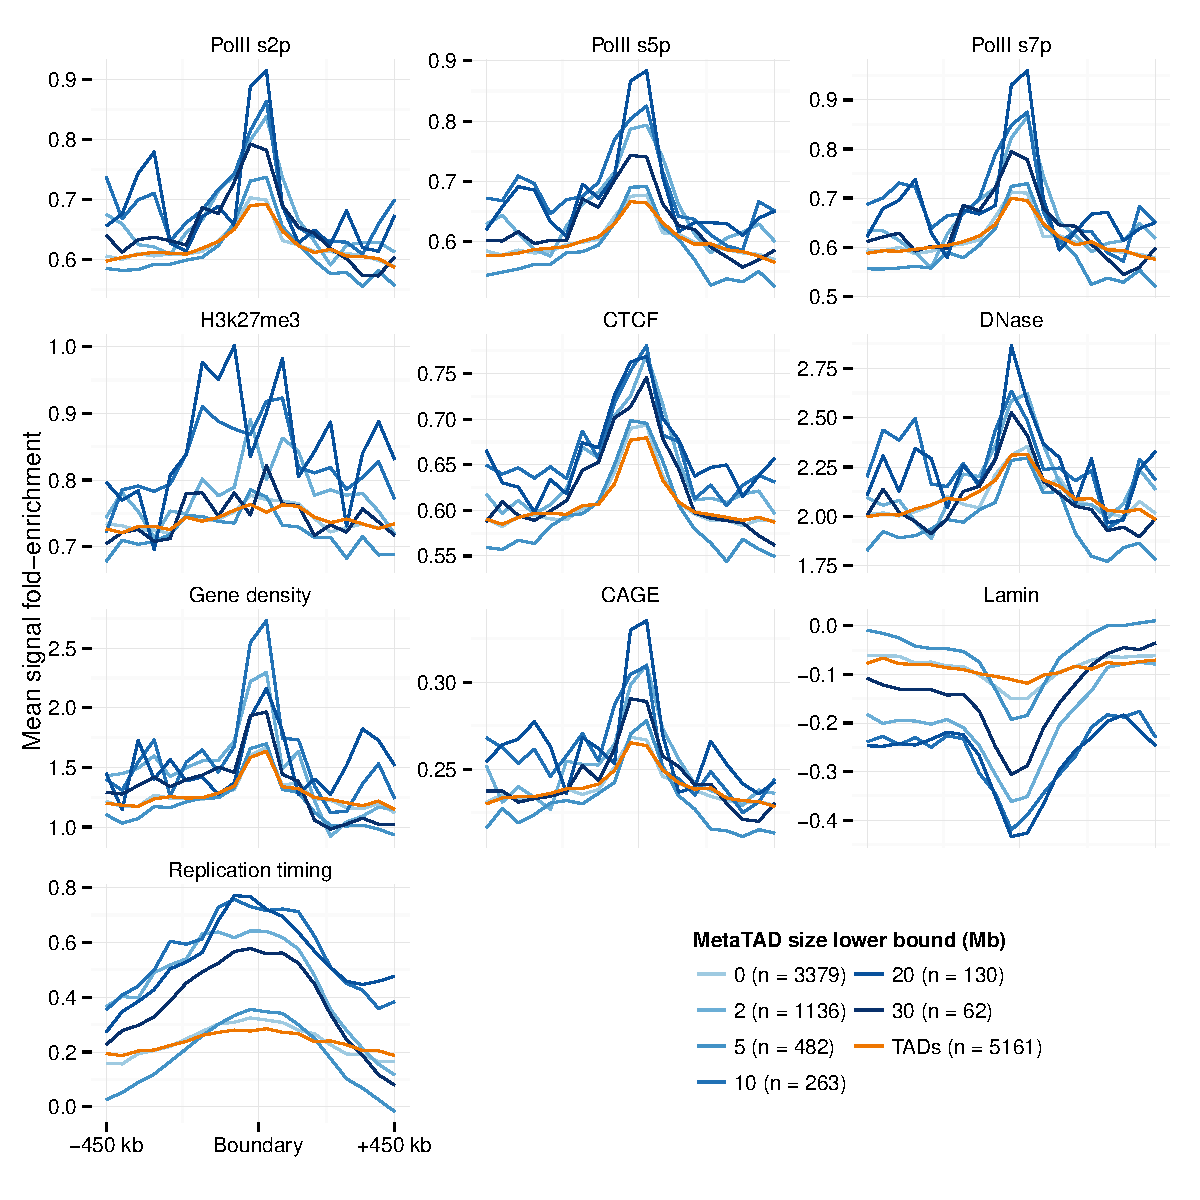
\includegraphics[width=4.5in]{metatad_cutoffenrich.pdf}
\captionsetup{width=\textwidth}
\caption[MetaTAD boundary enrichments and depletions with varying size selection.]{ {\bf MetaTAD boundary enrichments and depletions with varying size selection. }
Boundary average-o-grams are shown for TAD and metaTAD boundaries with variable lower bound cut-offs. Sample sizes for each threshold are shown in the legend (\emph{inset}).
}\label{fig:mtcutoffenrich}
\end{center}
\end{figure} 

\subsection{Lamina associated domains}\label{sec:mtlads}

In the previous section we report a colocation of metaTAD boundaries and lamina associated domains (LADs), and at a greater level than that observed with smaller TADs (Fig. \ref{fig:mtfeats}). This hints at an association between metaTADs and LADs which merits further investigation.

High resolution LAD data in mouse embryonic stem cells were retrieved from \citet{Peric-Hupkes2010} in the form of continuous measures of lamin-B1 association produced by the DamID technique, known to reflect proximity to the nuclear lamin.\cite{Pickersgill2006} This measure of lamina association was then processed in windows around each metaTAD and TAD boundary, and profiles were combined to form a heatmap (Fig. \ref{fig:mtlamin}).

\begin{figure}
\begin{center} 
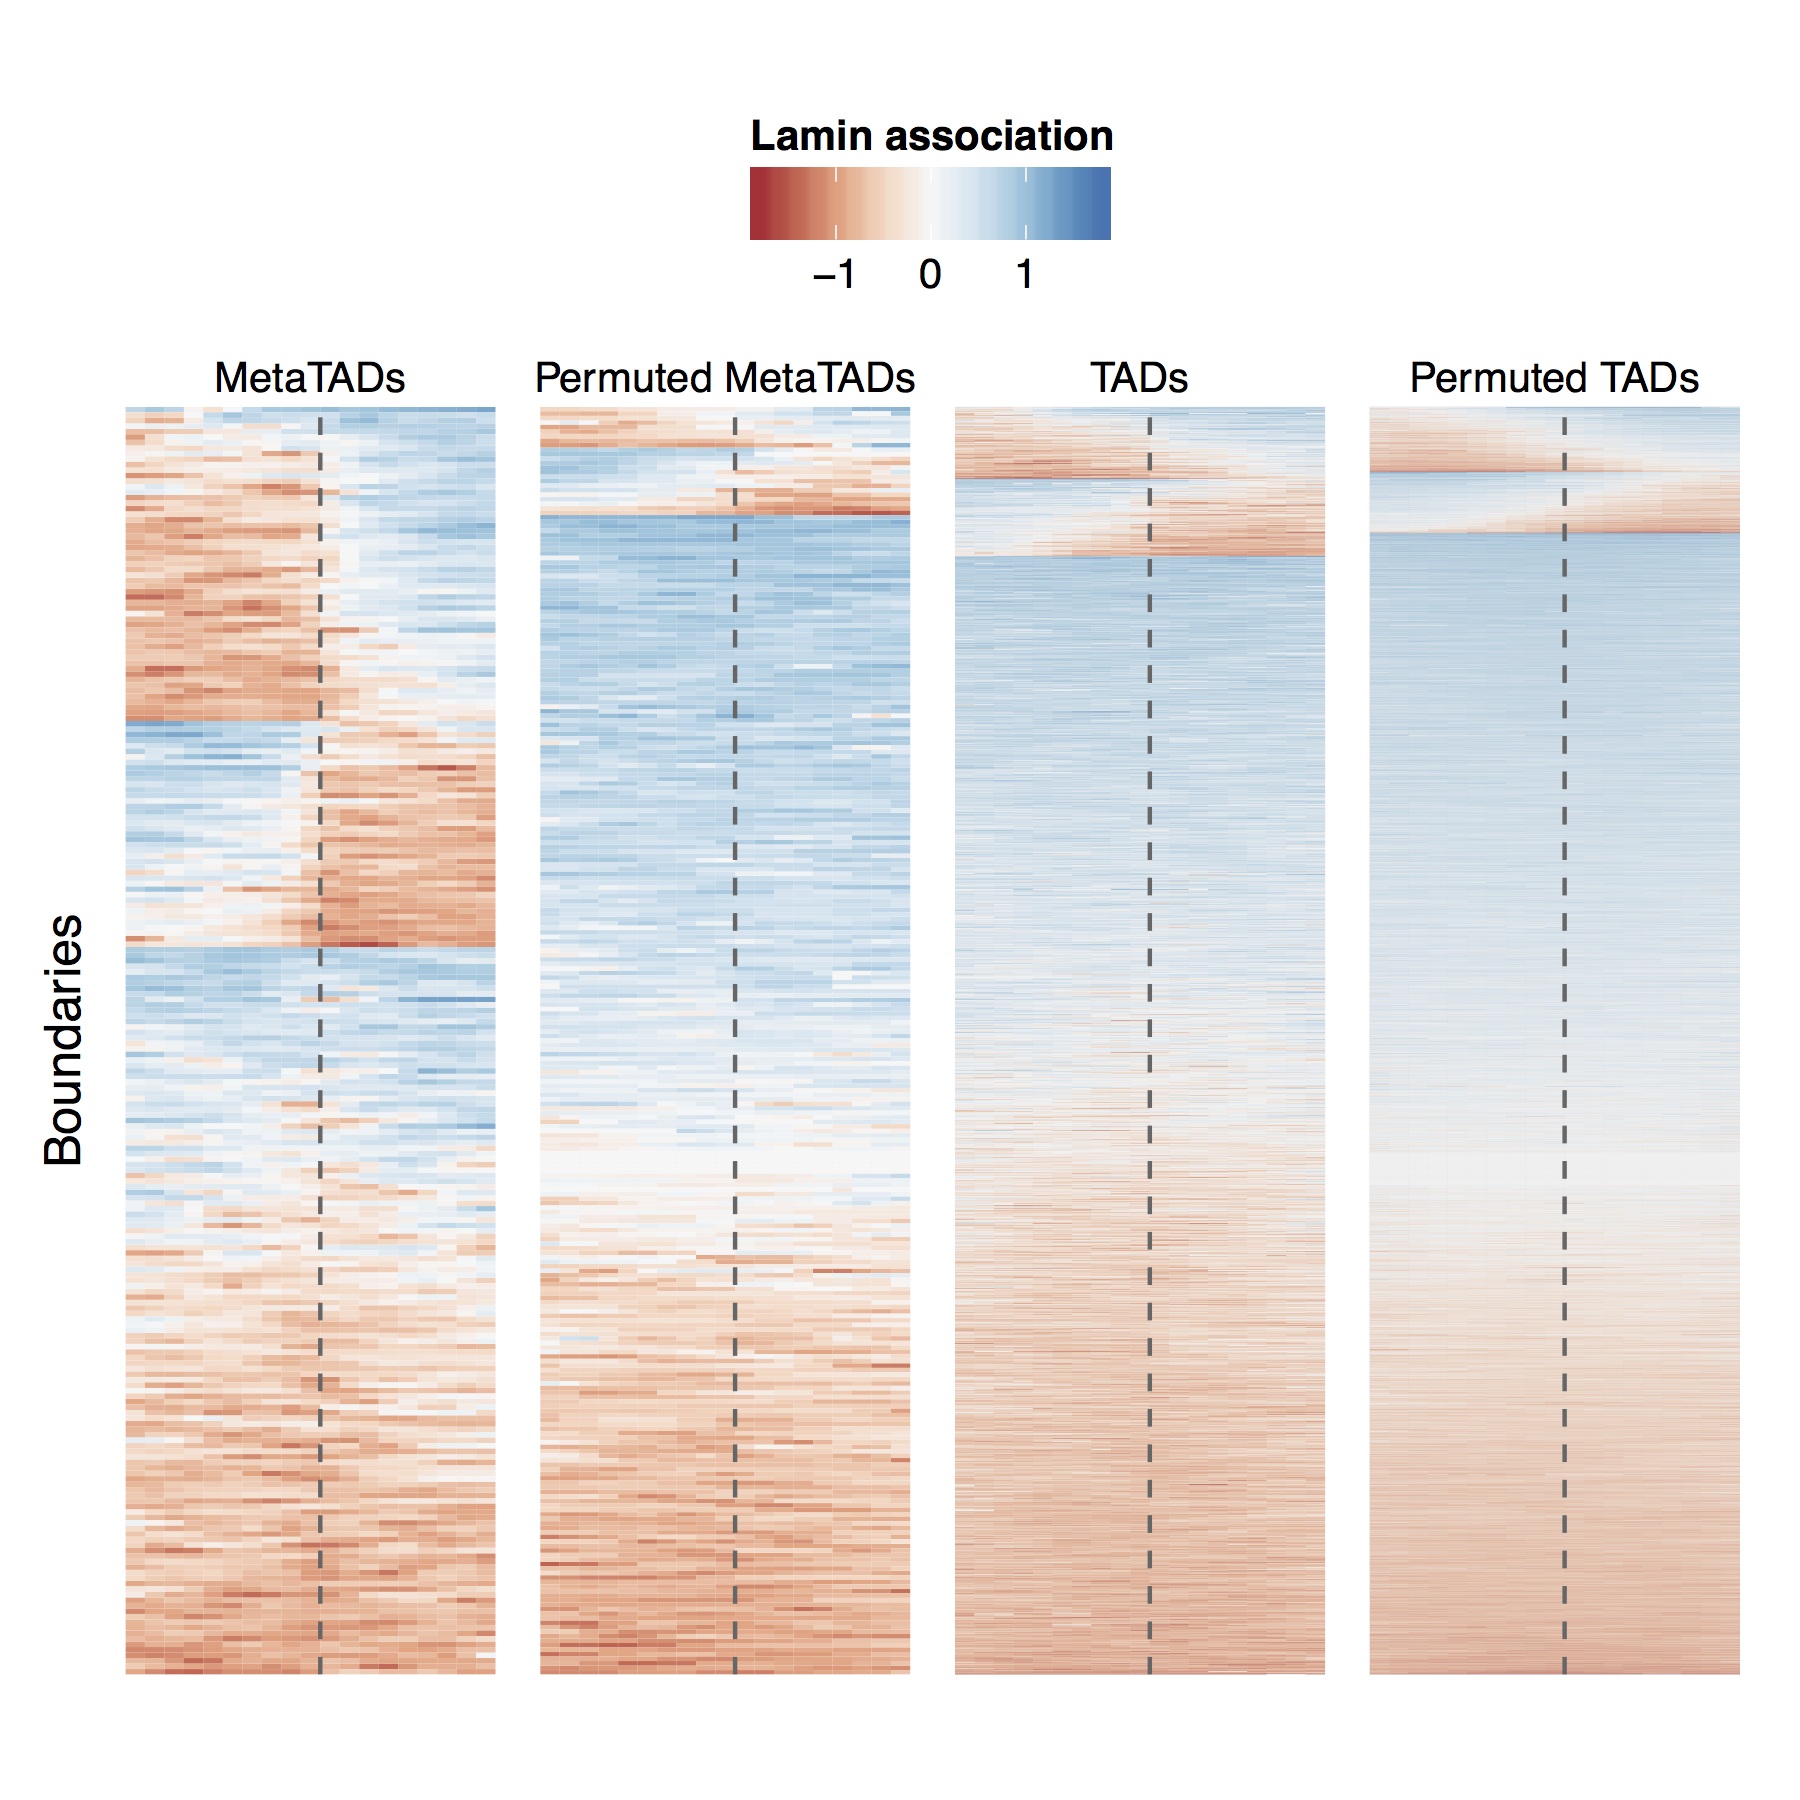
\includegraphics[width=4.5in]{mt_laminperm.png}
\captionsetup{width=\textwidth}
\caption[MetaTAD boundaries align with those of lamina associated domains.]{ {\bf MetaTAD boundaries align with those of lamina associated domains.}
Heatmaps of LaminB1 association microarray probe intensity values over MetaTAD boundaries (from domains of size 10 -- 40 Mb) and TAD boundaries, are displayed beside examples of circularly-permuted boundaries (Methods \ref{meth:metalad}). Profiles are shown $\pm450$ kb from each boundary.
}\label{fig:mtlamin}
\end{center}
\end{figure} 

Boundaries were seriated in order to separate out those that coincide with a LAD boundary, indicated by a transition in lamina association values. This was achieved by fitting a linear regression model across the lamina association profile of each boundary, then using a coefficient cutoff heuristic to select those that represent a boundary transition (Methods \ref{meth:metalad}).  Using this approach, we found a markedly large proportion of metaTAD boundaries ($43\%$) co-occur at a LAD boundary (Fig. \ref{fig:mtlamin}). The same comparison using TAD boundaries found a coincidence of just $12\%$. However LADs are large domains and there were over $5,000$ TADs called using these Hi-C data by our collaborators, thus in absolute numbers of boundaries this is still represents a large overlap.

To test the significance of these observations, we apply a permutation-based statistical test where our observed coincidences are compared with those produced by $1,000$ circular (per-chromosome) permutations (Methods \ref{meth:metalad}). We found that the metaTAD and LAD boundary coincidence is around a $2.7$-fold increase above null expectation (observed: $42.6\%$; expected: $15.8\%$; empirical $p$-value: $p < 1 \times 10^{-4}$; Fig. \ref{fig:mtsummary}). Meanwhile TAD boundaries were found to have a smaller, yet still significant, $1.2$-fold increase in coincidence with LAD boundaries relative to a null model (observed: $11.8\%$; expected: $9.5\%$; empirical $p$-value: $p < 1 \times 10^{-4}$; Fig. \ref{fig:mtsummary}).

\begin{figure}
\begin{center} 
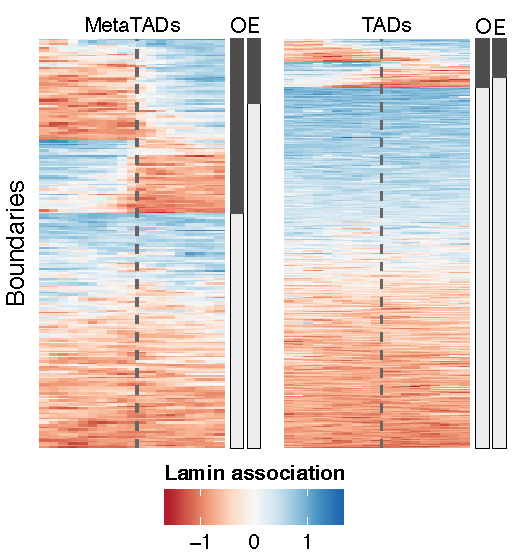
\includegraphics[width=2.5in]{mt_laminsummary.pdf}
\captionsetup{width=\textwidth}
\caption[ MetaTAD boundaries co-occur with LAD boundaries more often than is expected by chance. ]{ {\bf MetaTAD boundaries co-occur with LAD boundaries more often than is expected by chance. }
Heatmaps of lamina association over MetaTAD boundaries are shown as in Figure \ref{fig:mtlamin}. Sidebars labelled O and E reflect observed and expected proportions of metaTAD / LAD boundary overlaps (Methods \ref{meth:metalad}).
}\label{fig:mtsummary}
\end{center}
\end{figure} 

As with other enrichments (e.g. Fig. \ref{fig:mtcutoffenrich}), we went on to verify that this result was not specific to the choice of boundary size cutoff. Recall that as metaTADs are derived from TADs, selecting metaTADs within a size range is a trade-off between minimising overlap between boundaries assigned to TADs and metaTADs to enable more powerful comparison, while retaining a sufficiently large sample size of metaTAD boundaries (Section \ref{sec:metaVtad}). In the case of LAD--metaTAD coincidence, we again find this result is insensitive to the selection of domain size cutoff, and indeed that there is evidence for an increasing proportion of co-occurrence as we ascend the metaTAD hierarchy (Fig. \ref{fig:mtcutoffrange}).

\begin{figure}
\begin{center} 
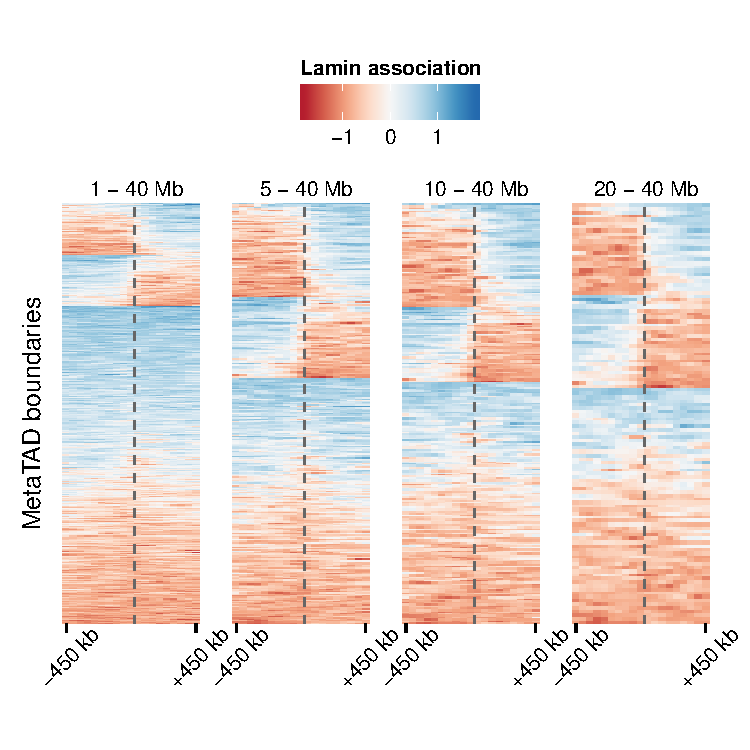
\includegraphics[width=5in]{mt_cutoffrange.pdf}
\captionsetup{width=\textwidth}
\caption[ MetaTAD--LAD coincidence increases at higher levels of the metaTAD hierarchy. ]{ {\bf MetaTAD--LAD coincidence increases at higher levels of the metaTAD hierarchy. }
Heatmaps of lamina association over MetaTAD boundaries are shown as in Figure \ref{fig:mtlamin}. Panels show the size selection cutoffs for metaTAD domains considered in each case.
}\label{fig:mtcutoffrange}
\end{center}
\end{figure} 

This result suggests again that metaTADs seems to offer useful perspectives onto higher order genome organisation. In this case, it appears TADs will often neatly aggregate within LADs and together these constitute what we observe as a metaTAD.

\subsection{Boundaries over a time series}

For the first time, our collaborator's applied the Hi-C technique over a differentiation time course from mouse embryonic stem cells, to neural progenitors and finally fully-differentiated neuron cells. Successive expression measures were also taken alongside this Hi-C data in the form of CAGE data, produced by the FANTOM5 consortium.\cite{fantom5} Together these datasets offer a unique perspective onto how higher order genome organisation varies with expression during differentiation. 

Collaborators explored changes in both the overall tree structure between timepoints, and aggregate expression changes between TADs and metaTADs at successive timepoints. They identified rewiring events in the metaTAD tree over the timecourse, and found corresponding changes in expression (\emph{data not shown}). Given metaTAD structures appear to differ and matched CAGE data exists for each timepoint, it was of interest to test how observed boundary enrichments for gene expression (Figs. \ref{fig:mtfeats}, \ref{fig:mtcutoffenrich}) might vary over this timecourse. 

\begin{figure}
\begin{center} 
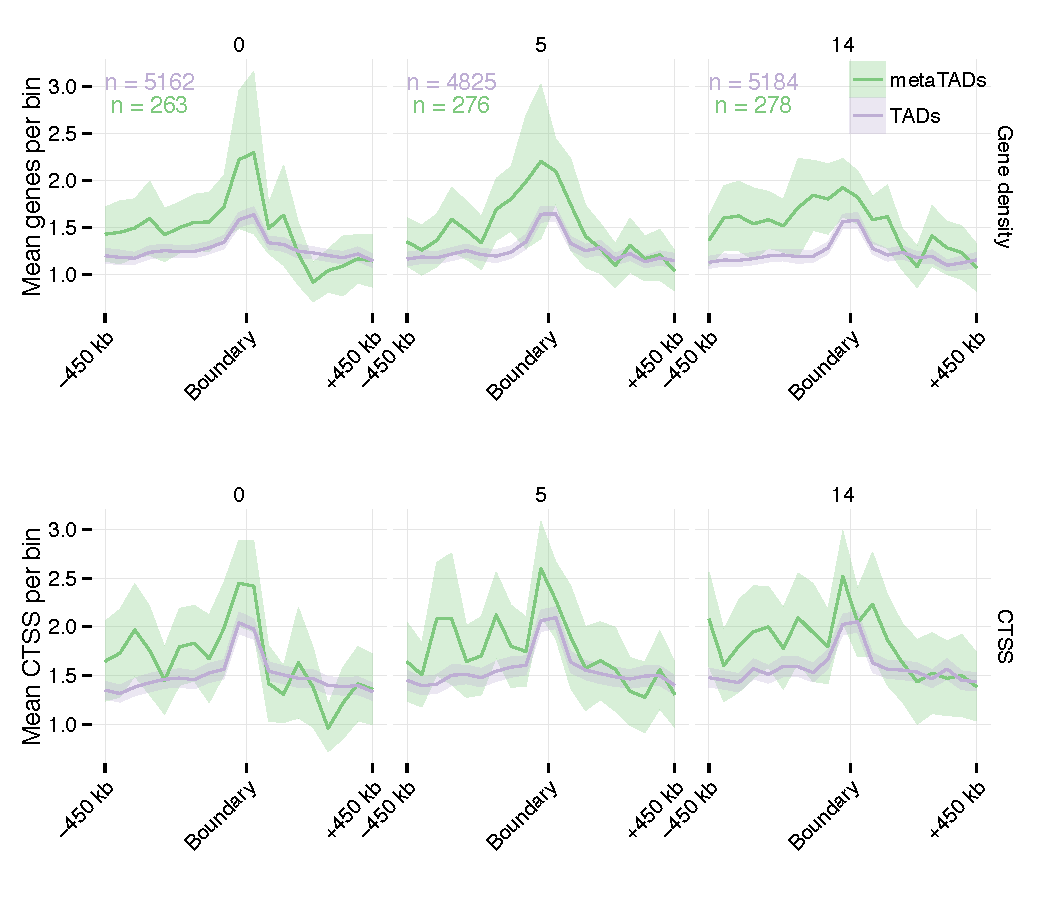
\includegraphics[width=4.5in]{mt_ts.pdf}
\captionsetup{width=\textwidth}
\caption[Observed enrichments persist over a time series.]{ {\bf Observed enrichments persist over a time series.}
CAGE-defined active TSS (CTSS) were counted per $50$ kb bin across each TAD and MetaTAD (10 -- 40 Mb) boundary and averaged (ribbons show $95\%$ confidence intervals of the mean). Gene densities refer to mean counts of annotated genes per bin, with an overlap of at least 250 bp (Methods \ref{meth:metadata}).
}\label{fig:mtts}
\end{center}
\end{figure} 

We find actively-transcribed CAGE-defined TSS (CTSS) to be consistently enriched over the shifting boundaries through the differentiation timecourse (Fig. \ref{fig:mtts}). We coupled this with a static measure of gene density in order to distinguish expression changes from genic overlap, however both series show similar patterns so it does not seem that boundary expression varies at a global scale over this timecourse. At each timepoint, peak heights over boundary bins suggest modestly stronger enrichments at metaTAD boundaries relative to TAD boundaries, as seen with other features (Fig. \ref{fig:mtfeats}). 

\section{Other boundaries}

\subsection{Giemsa bands}

% text (colin's?) from pre-submission old manuscript draft
A recent analysis of Hi-C datasets examined the hierarchy of nuclear compartment and TAD organisation in human HeLa cells across the cell cycle. They found that interphase and metaphase chromatin structure are highly distinct, such that the TADs and compartments observed here (e.g. Fig. \ref{fig:blowout}) are effectively abolished in metaphase.\cite{Naumova2013} This raises the question of how the structural organisation seen in (and often shared between) interphase cells is inherited through the cell cycle.

Human Giemsa metaphase banding (G-band) pattern data have been integrated with the human genome assembly, and although such data are widely used, they are also necessarily of low resolution.\cite{Furey2003} These G-band patterns are constant over human cell types at metaphase, but all traces of interphase higher order structure were reported to be absent at metaphase.\cite{Naumova2013} We would therefore not necessarily expect an agreement between G-bands, labelled in metaphase cells, and nuclear compartments, called from cell populations which were mostly in interphase. 

We examined the genome wide concordance of interphase compartment boundaries with metaphase G-band boundaries, relative to an expected distribution derived by permutation (Methods \ref{giemsa-band-comparison}). We found a significant, though modest, excess of compartment boundaries within close proximity of G-band boundaries, such that $13.9\%$ of compartment boundaries are within $500$ kb of a G-band boundary (expectation = $10.5\%$, K-S test: D $= 0.076$, p $< 3 \times10^{-12}$). This is seen for compartment boundaries calculated for all three cell types independently (a full comparison for GM12878 is shown in Figure \ref{fig:gbands2}). 

\begin{figure}
\begin{center} 
\makebox[\textwidth][c]{ 
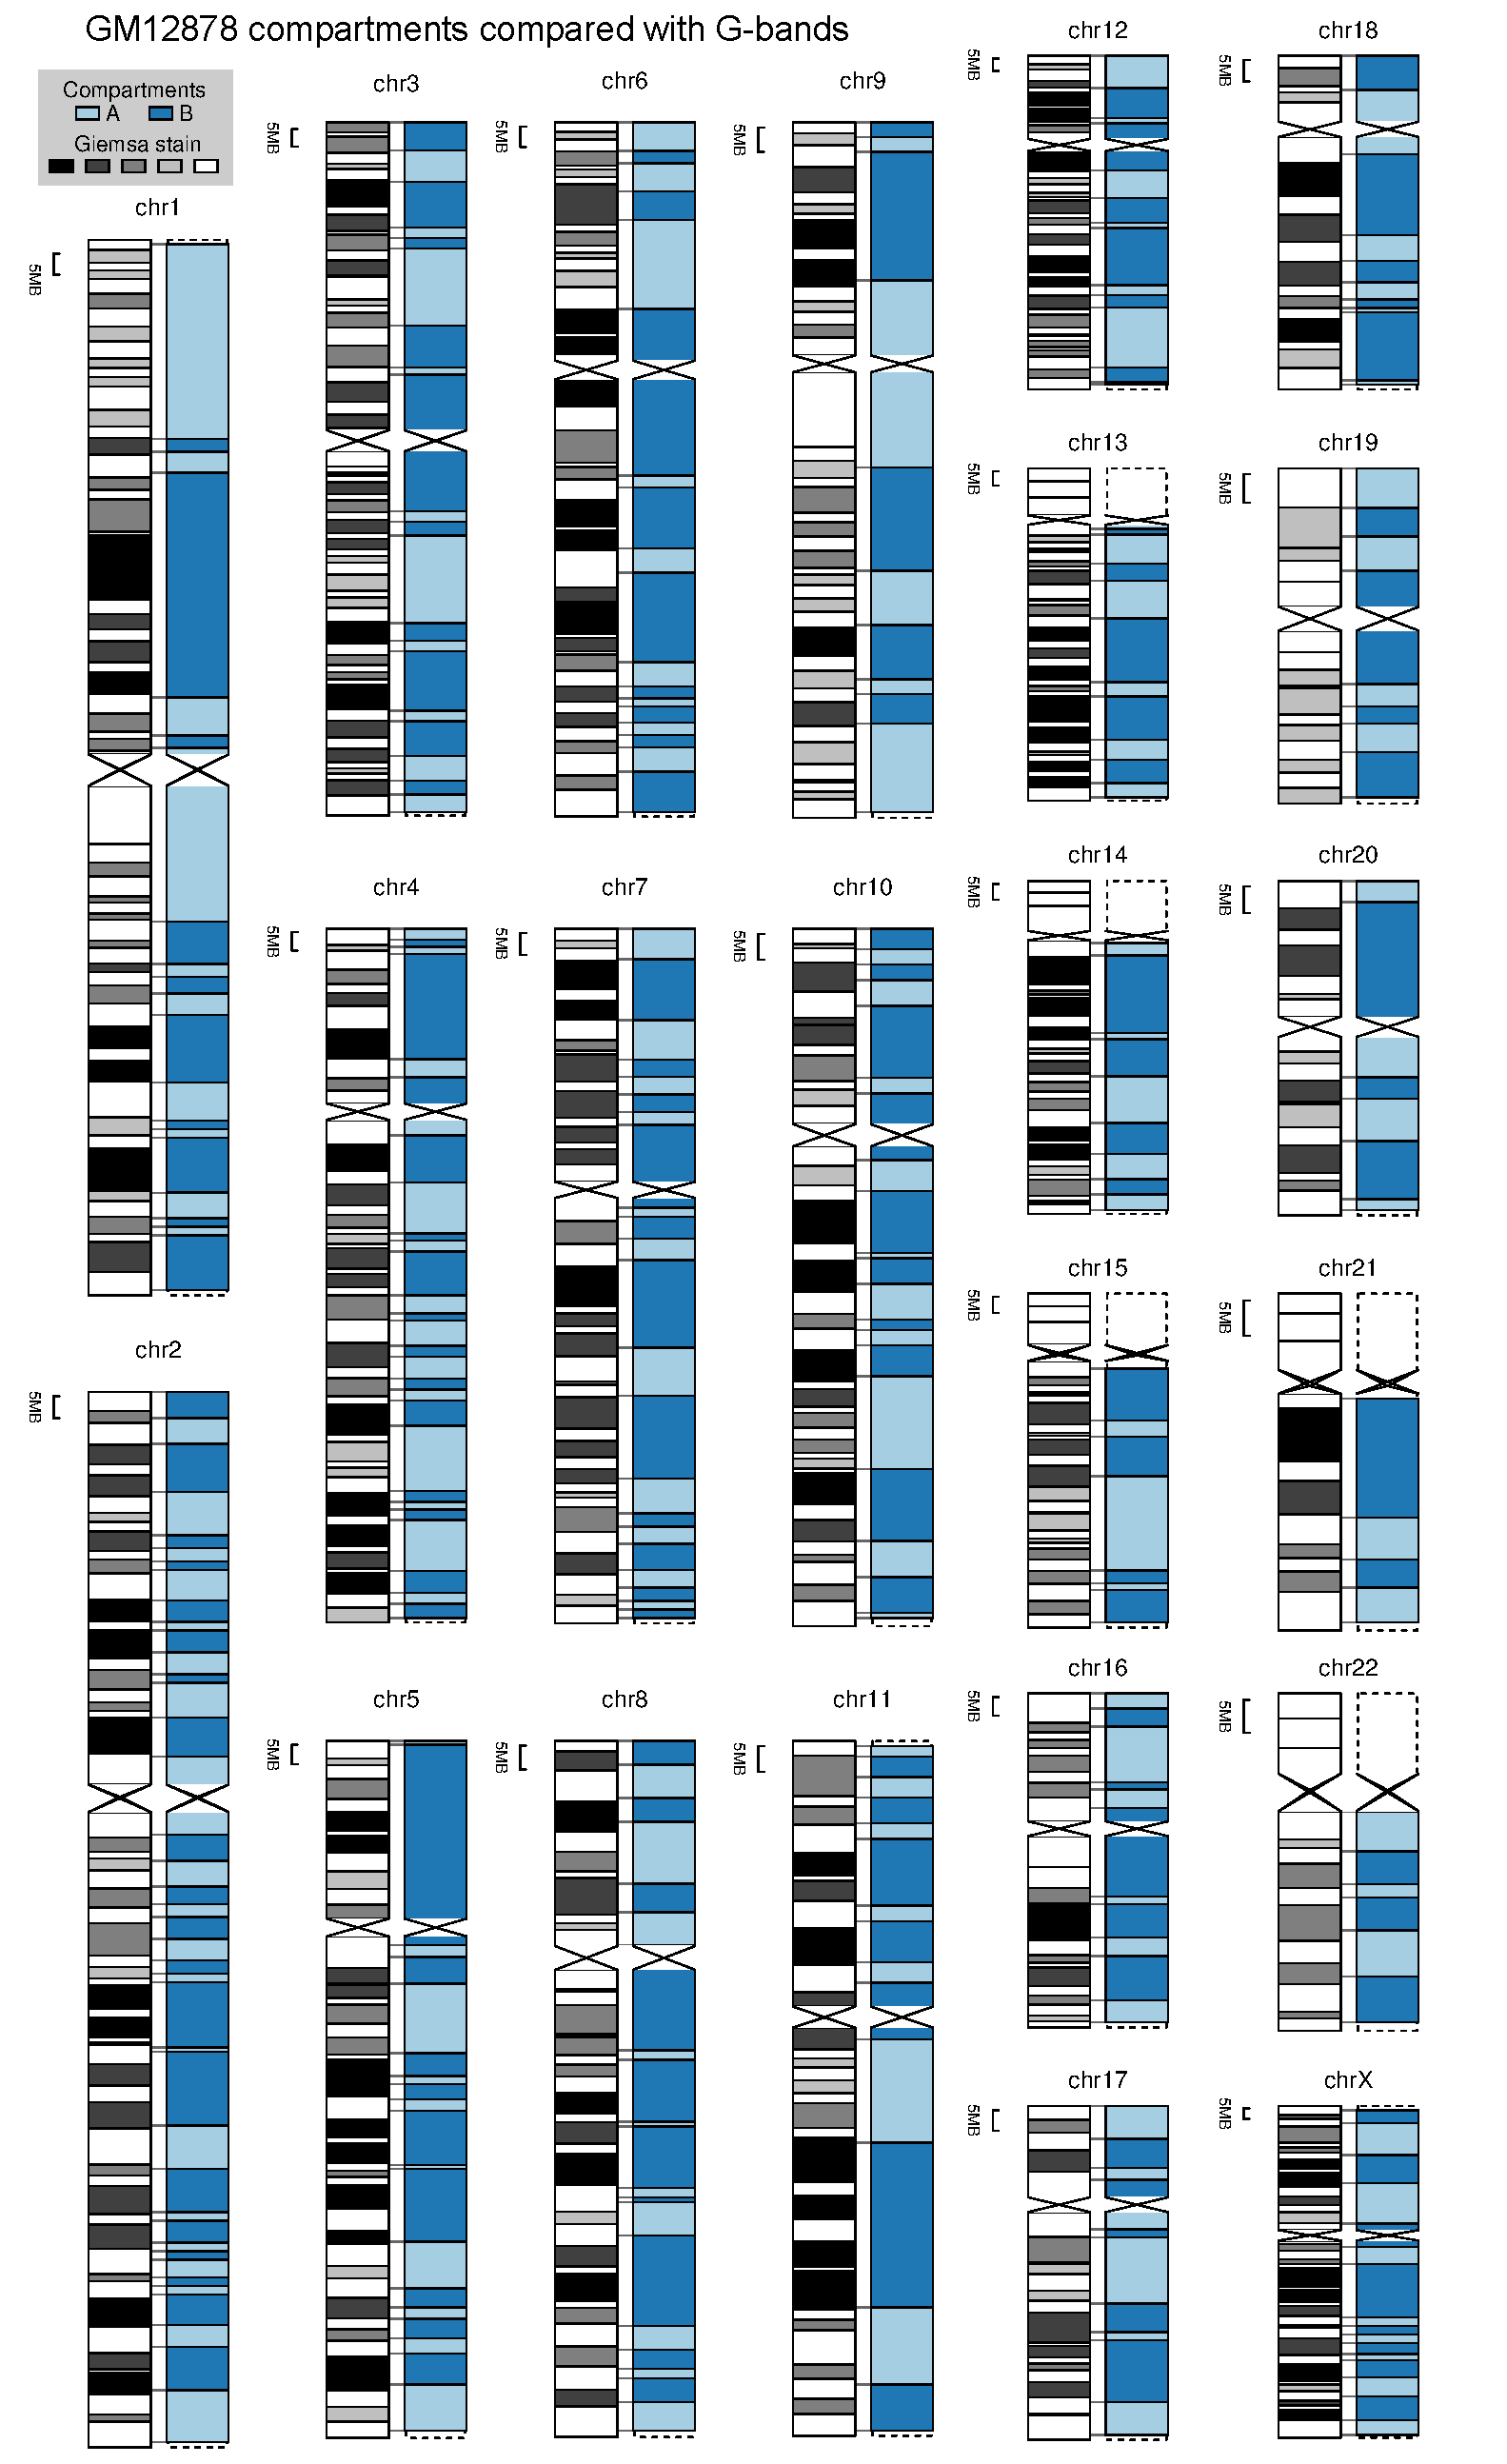
\includegraphics[width=5.7in]{gb_ideo.pdf}
}
\captionsetup{width=\textwidth}
\caption[Genome-wide agreement between Giemsa bands and A/B compartments..]{ {\bf Genome-wide agreement between Giemsa bands and A/B compartments. }
G-bands, assayed at metaphase, often correspond with interphase A/B compartments across all chromosomes. Data for cell type GM$12878$ is shown.
}\label{fig:gbands2}
\end{center}
\end{figure} 

The genome wide overlap of compartment A and B regions with particular G-band classes is nonrandom, and suggests a greater correspondence than that of simple boundary distances. Regions assigned to compartment A are significantly over-represented within lighter staining (especially G-negative) bands, while compartment B regions are over-represented in the most darkly staining (G-positive) bands (Fig. \ref{fig:gbands}). Approximately $40\%$ of the genome jointly occupies interphase compartment A as well as the lightly-stained \texttt{gneg} or \texttt{gpos25} metaphase G-bands, or occupies the interphase B compartment in addition to the well-stained \texttt{gpos75} or \texttt{gpos100} bands at metaphase (Fig. \ref{fig:gbands}). Similar trends are seen across all three cell types as expected given the high correlations seen in A/B compartment profiles between cell types (\emph{data not shown}). 

This agreement is not wholly unexpected given the known characteristics of G-negative and G-positive bands, with contrasting gene density, GC content and replication timing\cite{Furey2003} that is strongly reminiscent of the contrasts between interphase A and B compartments.\cite{Lieberman2009} Despite showing an association, these data agree with experimental evidence that many domain boundaries are not well preserved between interphase and metaphase. However there is evidence for relationships between the broad structural categories of compartments and G-bands which may reflect similarities in the degree of compaction throughout the cell cycle.

\begin{figure}
\begin{center} 
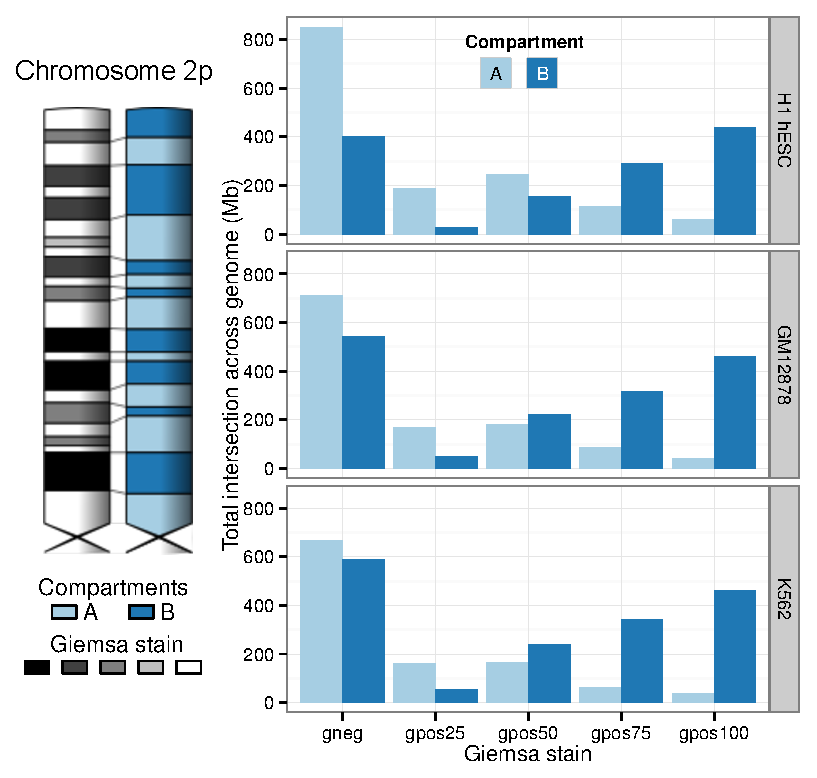
\includegraphics[width=3.8in]{gbands.pdf}
\captionsetup{width=\textwidth}
\caption[ Giemsa--stain bands correspond to A/B compartments.]{ {\bf Giemsa--stain bands correspond to A/B compartments.}
The correspondence between G-bands and A/B compartments is broken down into the five levels of Giemsa stain. A compartments largely match \emph{gneg} staining, while \emph{gpos75} and \emph{gpos100} are enriched in B compartments.
}\label{fig:gbands}
\end{center}
\end{figure} 

%\subsection{Superboundaries}
%
%Thus far compartment and TAD boundaries have been considered separately, however it is of interest to consider how these boundary regions interact across scales. Open questions remain about the co-occurence of these two boundary regions, and whether 


\ifstandalone
\begin{small}
\bibliography{/Users/benmoore/Documents/library,/Users/benmoore/Documents/customrefs}
\end{small}
\fi

\end{document}
